%%%%%%%%%%%%%%%%%%%%%%% file template.tex %%%%%%%%%%%%%%%%%%%%%%%%%
%
% This is a general template file for the LaTeX package SVJour3
% for Springer journals.          Springer Heidelberg 2010/09/16
%
% Copy it to a new file with a new name and use it as the basis
% for your article. Delete % signs as needed.
%
% This template includes a few options for different layouts and
% content for various journals. Please consult a previous issue of
% your journal as needed.
%
%%%%%%%%%%%%%%%%%%%%%%%%%%%%%%%%%%%%%%%%%%%%%%%%%%%%%%%%%%%%%%%%%%%
%
% First comes an example EPS file -- just ignore it and
% proceed on the \documentclass line
% your LaTeX will extract the file if required
\begin{filecontents*}{example.eps}
	%!PS-Adobe-3.0 EPSF-3.0
	%%BoundingBox: 19 19 221 221
	%%CreationDate: Mon Sep 29 1997
	%%Creator: programmed by hand (JK)
	%%EndComments
	gsave
	newpath
	20 20 moveto
	20 220 lineto
	220 220 lineto
	220 20 lineto
	closepath
	2 setlinewidth
	gsave
	.4 setgray fill
	grestore
	stroke
	grestore
\end{filecontents*}
%
\RequirePackage{fix-cm}
%
\documentclass{svjour3}                     % onecolumn (standard format)
%\documentclass[smallcondensed]{svjour3}     % onecolumn (ditto)
%\documentclass[smallextended]{svjour3}       % onecolumn (second format)
%\documentclass[twocolumn]{svjour3}          % twocolumn

%
\smartqed  % flush right qed marks, e.g. at end of proof
%
\usepackage{graphicx}
%
% \usepackage{mathptmx}      % use Times fonts if available on your TeX system
%
% insert here the call for the packages your document requires
%\usepackage{latexsym}
% etc.
\usepackage{amsmath,amsfonts,amssymb,amscd,xspace}
\usepackage{longtable}
\usepackage{booktabs}

% Hyperlinks
\usepackage[pdfpagemode={UseOutlines},bookmarks=true,bookmarksopen=true,
bookmarksopenlevel=0,bookmarksnumbered=true,hypertexnames=false,
colorlinks,linkcolor={blue},citecolor={blue},urlcolor={red},
pdfstartview={FitV},unicode,breaklinks=true]{hyperref}
\usepackage{hyperref}
\hypersetup{urlcolor=blue, colorlinks=true}  % 

\usepackage[english]{babel}
\usepackage{xcolor}
\usepackage[utf8]{inputenc} % tegnsetting i kildekoden
%\usepackage[T1]{fontenc}
%\usepackage[authoryear]{natbib}  % 
\usepackage[numbers]{natbib}
\usepackage{subcaption}
%\usepackage{algorithm}
%\usepackage[]{algorithm2e}
%\usepackage{algpseudocode} 
%\usepackage{program}
\usepackage[toc,page]{appendix}
\usepackage{bbm}


%
% please place your own definitions here and don't use \def but
% \newcommand{}{}
\newcommand{\E}{\ensuremath{\mathbb{E}}}
\newcommand{\Var}{\mathrm{Var}}
\newcommand{\Cov}{\mathrm{Cov}}
\newcommand{\Prob}{\ensuremath{\mathbb{P}}}
\newcommand{\Filtration}{\ensuremath{\mathcal{F}}}
\newcommand{\R}{\ensuremath{\mathbb{R}}}
\newcommand{\Complex}{\ensuremath{\mathbb{C}}}
%\newcommand{\intintens}{\mathrm{I}(v)}
%\newcommand{\intapprox}{\ensuremath{\mathcal{H}}}
\newcommand{\Lagr}{\mathcal{L}}
\newcommand{\norm}[1]{\left\lVert#1\right\rVert}
\newcommand{\cutoff}{\varsigma}
\newcommand*\mean[1]{\bar{#1}}
\newcommand{\target}{\ensuremath{r}}
\newcommand{\cRe}{\operatorname{\mathbb{R}e}}
\newcommand{\cIm}{\operatorname{\mathbb{I}e}}
%% START - Indenting in algorithms
%\newlength\myindent
%\setlength\myindent{2em}
%\newcommand\bindent{%
%	\begingroup
%	\setlength{\itemindent}{\myindent}
%	\addtolength{\algorithmicindent}{\myindent}
%}
%\newcommand\eindent{\endgroup}
%% END - Indenting in algorithms
\newtheorem{prop}{Proposition}
%\newtheorem{definition}{Definition}[section]
%
%\newcommand{\mathbbm}[1]{\text{\usefont{U}{bbm}{m}{n}#1}} % from mathbbm.sty

% article specific commands
\newcommand{\euler}{\hat{X}_t^{s1}}
\newcommand{\milstein}{\hat{X}_t^{s2}}
\newcommand{\schemethree}{\hat{X}_t^{s3}}
\newcommand{\spa}{\textt}


% Insert the name of "your journal" with
% \journalname{myjournal}
%
\begin{document}

\title{Likelihood estimation of jump diffusions%\thanks{Grants or other notes
%about the article that should go on the front page should be
%placed here. General acknowledgments should be placed at the end of the article.}
}
%\subtitle{Do you have a subtitle?\\ If so, write it here}

%\titlerunning{Short form of title}        % if too long for running head

\author{Berent Å. S. Lunde         \and
        Hans J. Skaug \and
        Tore S. Kleppe
}

\authorrunning{B. Lunde \and H. J. Skaug} % if too long for running head

\institute{Berent Ånund Strømnes Lunde \at
		University of Stavanger \\
		Tel.: +47-4725-8605\\
		%              Fax: +123-45-678910\\
		\email{berent@nql.no}  
%             \emph{Present address:} of F. Author  %  if needed
           \and
           S. Author \at
              second address
}

\date{Received: date / Accepted: date}
% The correct dates will be entered by the editor


\maketitle

\begin{abstract}
This article considers the problem of likelihood-based parameter estimation for time-homogeneous jump-diffusion processes. 
The problem is that there often is no analytic solution to the stochastic differential equations driving the process.
Thus, the transition density of the process is unknown.
In this article we build on the solution diffusions presented in \citet{preston2012approximation} and extended in \citet{zhang2016approximation}, where the transition density of a time-homogeneous jump diffusion process is approximated by inverting an approximate characteristic function.
We reproduce the results found here, and extend the analysis with maximum likelihood estimation for benchmark processes.
The conditions for which likelihood estimation is feasible and do not suffer under non-identifiability are provided.
We investigate different numerical inversion techniques for both diffusions and jump diffusions. the use of direct saddlepoint approximation, renormalized saddlepoint, and quadrature rules.
We find that, in practice, care must been taken when choosing the numerical inversion technique for both diffusions and jump diffusions.
To this end, we propose a numerically stable inversion algorithm, containing the best properties of saddlepoint techniques and quadrature integration.
Simulation studies are executed to reveal potential bias of the different schemes.
As a proof of concept, the likelihood estimation method is applied to the analysis of stock prices modelled as nonlinear stochastic differential equations, with and without jumps.
Finally we briefly analyse some models for stochastic volatility.
\keywords{Jump diffusions \and Likelihood estimation \and Inverse Fourier transform \and Saddlepoint approximation \and Ito Taylor expansions}
% \PACS{PACS code1 \and PACS code2 \and more}
% \subclass{MSC code1 \and MSC code2 \and more}
\end{abstract}

\section{Introduction}
\label{sec::intro}
Itô calculus, first proposed by Kiyoshi Itô and popularized by the elegant solution to the problem of pricing options proposed in \citet{black1973pricing}, has become the focus of many studies.
It has applications to many fields of research, such as physics and chemistry, but is perhaps mostly reckoned with in the context of mathematical finance. 
Stochastic differential equations, governing the Itô process, are used to model a wide variety of objects in mathematical finance, from stock prices to stochastic volatility, as in the Heston stochastic volatility model \citep{heston1993closed}. A good introduction to the subject can be found in \citet{oksendal2003stochastic}. 
Stochastic differential equations are often problematic in the sense that it is, in general, not known how to solve them analytically.
This is a problem for pricing formulas in finance, for simulation of the process, and for inference about parameters. 
A solution is to estimate the solution with a series expansion of the driving equation, similar to that of the familiar Taylor expansions, indeed these series expansions are called \textit{Itô-Taylor expansions}. A rigorous development and application of the Itô-Taylor expansions can be found in \citet{kloeden1992numerical}.\\

Models in finance are often modelled under the hypothesis that markets are efficient. This implies that all valuable information for a stock is already embedded in the stock price. In practice, the expectation of future values (and all other aspects) of the price of the stock is the same whether you condition on the current state, or whether you condition on all previous states. For these reasons, models will typically have the Markov property, and in the case of continuous time models, they are typically specified by the time-homogeneous stochastic differential equation:
\begin{align}\label{ItoSDE}
dX_t=\mu(X_t;\theta)dt+\sigma(X_t;\theta)dW_t +c(X_{t^-},\xi_{N_{t^-}+1})dN_t.
\end{align}
Given discrete observations $\left\{X_{t_i}\right\}$ of the process, where $i$ ranges from $i=1,\ldots,n$, and due to the Markov property of the Itô process, the log-likelihood can be written as:
\begin{align}\label{Chap1 jll}
l(\theta|x_{t_1},...,x_{t_n})=\sum_{i=2}^{n}\log p(x_{t_i}|x_{t_{i-1}},\theta),
\end{align}
where
\begin{align}
p(x_{t_i}|x_{t_{i-1}},\theta)=\frac{d}{dx_{t_i}}P(X_{t_i}<x_{t_i}|X_{t_{i-1}}=x_{t_{i-1}},\theta)
\end{align}
is the all important transition density \citep{preston2012approximation, lindstrom2007estimating}.  \\

The problem of doing inference about parameters of diffusion processes where the transition density is not known, has a variety of solutions. 
Likelihood-based estimation needs the transition density to build the likelihood, and various methods have therefore been developed, either to approximate it or to find it exactly.
\citet{preston2012approximation} place these approaches for pure diffusions into three categories.
The first approach involves obtaining the transition density via the Kolmogorov equations for the transition density \citep{lindstrom2007estimating}.
The second involves simulating the process, either approximately \citep{durham2002numerical} or exact \citep{beskos2006exact}.
A third alternative is to replace the continuous process with a discrete approximation where it is possible to find the transition density \citep{shoji1998estimation, ait1999transition}. 
This third solution is well applicable when the time steps between the observations are small, and this bodes well for financial data. In addition, it is particularly suited for adding jumps, as shown in \citet{zhang2016approximation}.\\

In this article we follow and extend the work done in \citet{preston2012approximation}, which falls into the third category: replacing the continuous process with a discrete version. The method in this paper can be broken down into the following three steps:
\begin{enumerate}
	\item Develop an Itô-Taylor expansion of the sample path.
	\item Calculate the moment generating function of the retained terms in the expansion.
	\item Approximate the inverse Fourier transform by a saddlepoint approximation to the transition density.
\end{enumerate}
% \cite{preston2012approximation} \\
The extension of this method to a time-homogeneous jump-diffusion process is possible due to the independence between the jump components and the pure diffusion parts.
Such an extension is already done by \citet{zhang2016approximation}, where the approximation in step 3 is carried out by the FFT algorithm.

The two sections following the introduction are concerned with the mathematical tools necessary to understand the method in \citet{preston2012approximation}, which we shall call the \textit{Itô-Taylor saddlepoint approximation} (ITSPA). 
In chapter \ref{sec::ito_taylor} we explain the Itô-Taylor expansions, used for expanding the sample path of the process, 
and we provide conditions for which the likelihood optimisation do not suffer from non-identifiability.
In chapter \ref{sec::ift} we discuss approximations of the inverse Fourier  transform of the characteristic function, such as the saddlepoint approximation, and we propose a numerically stable IFT approximation, retaining the best parts of the saddlepoint approximation and Gaussian quadrature rules.
% DO  BELOW IN SECTION 2 -- MENTION TMB AND AUTODIFF::
%We continue in chapter \ref{Chapter4} with the extensions of the ITSPA to jump-diffusions, and the refinement of the method in \citet{zhang2016approximation}.
%In chapter \ref{Chapter5} we discuss the benefits of the newly developed Template Model Builder (TMB) package, which by utilizing the techniques of automatic differentiation allows for exact numerical derivatives of the likelihood, making the optimization faster and more robust.
%We also extend the TMB package with some features, allowing us to implement the methods in chapter \ref{Chapter4}. 
Chapter \ref{sec::numerical_results} presents numerical results for benchmark processes using the implemented methods.
Plotted transition densities and numerical results from simulated likelihood-based analysis are used to compare the discretization schemes, the methods,  and refinements such as renormalization of the saddlepoint approximation.
Chapter \ref{sec::case_studies} is devoted to two case studies: the study of stock prices as a nonlinear process versus a linear process, and comparisons of stochastic volatility models.
In chapter \ref{sec::discussion} we conclude and comment on the results.\\

\section{Itô-Taylor expansions and discretization schemes}
\label{sec::ito_taylor}

In this section we will go through the derivation of the discretization schemes via the Itô-Taylor expansions.
We assume familiarity with the Brownian motion, the Itô integral, and Itô lemma.

\subsection{Itô Taylor expansions}
\label{sec_sub_ito_taylor}
Consider the two first terms on the right side of \textit{stochastic differential equation} (SDE) \eqref{ItoSDE}, which is shorthand for the integral equation,
\begin{align}\label{integral_ito}
X_t=X_{t_0}+\int_{t_0}^{t}\mu(X_s;\theta)ds+\int_{t_0}^{t}\sigma(X_s;\theta)dW_s.
\end{align}
The first integral is a standard deterministic integral, while the second is the \textit{Itô Integral}.
For properties of the Itô integral, see \citet[Chapter 3.2, p.~30]{oksendal2003stochastic}.
To handle another stochastic process, defined as a function of the solution, $Y_t= f(t,X_t)$, we need a stochastic analogue to the chain rule.
This is precisely what Itô's Lemma gives us.
\begin{theorem}\label{thorem; Ito lemma}
	Let $X_t$ be an Itô process satisfying the SDE \ref{integral_ito}.
	%\begin{align}
	%dX_t=\mu_tdt+\sigma_tdW_t.
	%\end{align}
	If $f(t,x)$ is a twice continuously differentiable function on $[0,\infty)\times\mathbb{R}$, then
	$
	Y_t=f(t,X_t)
	$
	is again an Itô process, and
	\begin{align}
	dY_t=\frac{\partial f}{\partial t}(t,X_t)dt+\frac{\partial f}{\partial x}(t,X_t)dX_t+
	\frac{1}{2}\frac{\partial^2 f}{\partial x^2}(t,X_t)\left(dX_t\right)^2,
	\end{align}
	where $(dX_t)^2$ is computed according to the following rules:
	\begin{align}
	dt dt=dt dW_t = dW_t dt = 0,\,\, dW_tdW_t=dt.
	\end{align}
\end{theorem} \citep{oksendal2003stochastic}

Itô's lemma can be used in a recursive manner to obtain expansions, similar to the familiar Taylor expansions, for diffusion processes governed by a SDE.
These expansions are called Itô-Taylor expansions and are very valuable in simulation and approximation of solutions of SDEs. 
We will limit ourselves to sketch how the expansions can be obtained in the case of an one-dimensional SDE. We do however note that expansions exist for multidimensional diffusion processes, and also for SDEs with jumps, see \citet{platen2010numerical}.
For an in-depth study of the Itô-Taylor expansions and their use, we refer to \citet{kloeden1992numerical}, from which the material in the following section is taken.

Before obtaining the Itô-Taylor series expansions, we define the following operators, to be used throughout the section:
\begin{align}
L^0&=\frac{\partial}{\partial t}
+\mu\frac{\partial}{\partial x}+\frac{1}{2}\sigma^2\frac{\partial^2}{dx^2},\\
L^1&=\sigma\frac{\partial}{\partial x}.
\end{align} 
Applying these operators in theorem \ref{thorem; Ito lemma}, we get Itô's lemma in operator form:
\begin{align}\label{ItoMultidimOperForm}
Y_t&=Y_{t_0}+\int_{t_0}^{t}L^0fds+\int_{t_0}^{t}L^1fdW_s.
\end{align}
Applying this twice to the right-hand side of equation \eqref{integral_ito},  first with $f(t,x)$ as $\mu(t,x)$ and then with $f(t,x)=\sigma(t,x)$, we have
\begin{align}
X_t&=X_{t_0}+\int_{t_0}^{t}
\left[
\mu(t_0,X_{t_0})+\int_{t_0}^{s}L^0\mu(\tau,X_\tau)d\tau \right.\notag\\
&	\left.+\int_{t_0}^{s}L^1\mu(\tau,X_\tau)dW_\tau
\right]ds
+\int_{t_0}^{t}\Bigg[ \sigma(t_0,X_{t_0})   \Bigg.\notag\\
&+\left.
\int_{t_0}^{s}L^0 \sigma(\tau,X_\tau)d\tau
+\int_{t_0}^{s}L^j\sigma(\tau,X_\tau)dZ_\tau^j
\right]dW_s.
\end{align}
Let $I_{i_1,i_2,...,i_k}$ represent the multiple It\^o integral, defined as
\[  I_\alpha = \left\{
\begin{array}{ll}\label{multiple_ito_integral}
1 & \text{if } k=0, \\
\int_{t_0}^{t}I_{\alpha^-} ds & \text{if } k\geq 1 \text{ and } \alpha_k=0,\\
\int_{t_0}^{t}I_{\alpha^-} dW_s & \text{if } k\geq 1 \text{ and } \alpha_k= 1,\\
\end{array} 
\right. \]
where $\alpha = (\alpha_1,\alpha_2,...,\alpha_k)^T$ is a $k$-dimensional vector of zeros and ones, and  $\alpha^-$ denotes the multi-index that can be obtained by deleting the last component of $\alpha$. For example,
\begin{align}
I_{0,1,0}=\int_{0}^{t}I_{0,1} ds_1 = \int_{0}^{t}\int_0^{s_1}I_{0}   ds_2ds_1    =\int_{0}^{t}\int_0^{s_1}\int_0^{s_2}ds_3dW_{s_2}ds_1.
\end{align}

Applying this notation, we have
\begin{align}
X_t&=X_{t_0} + \mu(t_0,X_{t_0})I_0+\sigma(t_0,X_{t_0})I_1 \notag \\
&+\int_{t_0}^t\left[
\int_{t_0}^{s}L^0\mu(\tau,X_\tau)d\tau
+\int_{t_0}^{s}L^1\mu(\tau,X_\tau)dE_\tau
\right]ds \notag \\
&+\int_{t_0}^t\left[
\int_{t_0}^{s}L^0\sigma(\tau,X_\tau)d\tau
+\int_{t_0}^{s}L^1\sigma(\tau,X_\tau)dW_\tau
\right]dZ_s.
\end{align}
We continue with the application of Itô's lemma in operator form \eqref{ItoMultidimOperForm}, now applied to the functions
$ L^0\mu$, 
$L^1\mu$, 
$L^0\sigma$ ,
and $L^1\sigma$, and again to the newly obtained functions 
$ 
L^0L^0\mu$, 
$L^1L^0\mu$, 
$L^0L^1\mu$, 
$L^1L^1\mu$, 
$L^0L^0\sigma$, 
$L^1L^0\sigma$, 
$L^0L^1\sigma$, and
$L^1L^1\sigma$,
to acquire the It\^o-Taylor expansion
\begin{align}
X_t&=X_{t_0}+\mu(t_0,X_{t_0})I_0+\sigma(t_0,X_{t_0})I_1\notag\\
&+L^0\mu(t_0,X_{t_0})I_{0,0}+L^1\mu(t_0,X_{t_0})I_{1,0}\notag\\
&+L^0\sigma(t_0,X_{t_0})I_{0,1}+L^1\sigma(t_0,X_{t_0})I_{1,1}\notag\\
&+L^0L^0\mu(t_0,X_{t_0})I_{0,0,0}+L^1L^0\mu(t_0,X_{t_0})I_{1,0,0}\notag\\
&+L^0L^1\mu(t_0,X_{t_0})I_{0,1,0}+L^1L^1\mu(t_0,X_{t_0})I_{1,1,0}\notag\\
&+L^0L^0\sigma(t_0,X_{t_0})I_{0,0,1}+L^1L^0\sigma(t_0,X_{t_0})I_{1,0,1}\notag\\
&+L^0L^1\sigma(t_0,X_{t_0})I_{0,1,1} + L^1L^1\sigma(t_0,X_{t_0})I_{1,1,1}+R,
\end{align}
where $R$ denotes the remainder term.

\subsection{Discretization schemes}
We now construct numerical integration schemes based upon the Itô-Taylor approximations developed in section \ref{sec_sub_ito_taylor}.
The first obstacle is the calculation of the first Itô integrals \eqref{multiple_ito_integral}.
We here state the results. 
The proof of the ones involving Brownian motions can be found in appendix \ref{AppendixB}.
For the first integrals, with $\alpha$ having two or fewer indices, we have
\begin{align}\label{solved_ito_integrals}
I_0&=\int_{0}^{t}ds=t,\notag\\
I_1&=\int_{0}^{t}dW_s=W_t=J_1,\notag\\
I_{0,0}&=\int_{0}^{t}\int_{0}^{s_1}ds_2ds_1=\frac{1}{2}t^2,\notag\\
I_{1,0}&=\int_{0}^{t}\int_{0}^{s_1}dW_{s_2}ds_1=\int_{0}^{t}W_{s_1}ds_1=J_2,\notag\\
I_{0,1}&=\int_{0}^{t}\int_{0}^{s_1}ds_2dW_{s_1}=\int_{0}^{t}s_1dW_{s_1}=tJ_1-J_2,\notag\\
I_{1,1}&=\int_{0}^{t}\int_{0}^{s_1}dW_{s_2}dW_{s_1}=\frac{1}{2}\left(J_1^2-t\right),
\end{align}
where the $J_i$'s are defined as $J_1=W_t$ and $J_2=\int_0^tW_sds$.
We note that the vector $\left( J_1,J_2 \right)^T$ has mean and covariance matrix
\begin{align}
\E \begin{pmatrix}
J_1\\J_2
\end{pmatrix} =
\begin{pmatrix}
0\\
0
\end{pmatrix},\,\,\,
\Var \begin{pmatrix}
J_1\\J_2
\end{pmatrix} =
\begin{pmatrix}
t & \frac{1}{2}t^2\\
\frac{1}{2}t^2 & \frac{1}{3}t^3, 
\end{pmatrix}
\end{align}
respectively. In addition, $J_1$ and $J_2$ are Gaussian \citep{preston2012approximation}.

There exist conditions under which an Itô-Taylor expansion attains a given order of strong convergence. 
These can be found in \citet[chapter 5]{kloeden1992numerical}. 
For the multiple Itô integrals \ref{multiple_ito_integral} $I_\alpha$, let $l(\alpha)$ denote the number of components in $\alpha$ and let $n(\alpha)$ denote the number of zero components. In the case of an one-dimensional SDE, all non-zero components are one. Then a scheme attains strong convergence of order $\gamma$ if it includes all terms with $\alpha$ satisfying $l(\alpha)+n(\alpha)\leq 2\gamma$ \citep{preston2012approximation}.

We will present three different schemes, the Euler-Maruyama scheme of strong order 0.5, the Milstein scheme of strong order 1.0, and a third scheme that can attain strong order 1.5. 
These schemes are presented in \citet{preston2012approximation}. 
In addition to these three schemes, there is a fourth one of strong order 2.0 presented here.
But this scheme involves a transformation to obtain unit diffusion. 
This is problematic for the intended extension to a more general jump-diffusion process and is therefore not considered here.

Following \citet{preston2012approximation}, we will consider time-homogeneous processes so that the drift and diffusion coefficients will only depend upon the state $X_t$ of the process at time $t$. 
We use $\mu$ and $\sigma$ to denote the drift and diffusion processes evaluated at the left point of the time interval, and primes to indicate derivatives. 
As an example:
\begin{align}
\mu=\mu\left.\left(X_t\right)\right|_{X_{t_0}},
\text{ and }
\sigma''=\left.\frac{\partial^2}{\partial x^2}\sigma\left(X_t\right)\right|_{X_{t_0}}.
\end{align}

\subsubsection{Scheme 1: The Euler-Maruyama Scheme}
The \textit{Euler-Maruyama Scheme} is the easiest and most used discretization based on the Itô-Taylor expansions \eqref{Chap2 Sec2}.
It attains strong order of convergence $0.5$ in general, but if the diffusion coefficient is constant, it attains strong order $1.0$ \citep{kloeden1992numerical}.
It provides good numerical results in the cases of simple processes with nearly constant drift and diffusion coefficients.
However, for processes with nonlinear coefficients, higher order schemes might be preferred.
In the one-dimensional case, it is of the form
\begin{align}\label{Chap4 Sec1.1 euler scheme}
X_t=X_{t_0}+\mu I_0+\sigma I_1,
\end{align}
which is Gaussian due to the $I_1$-term.
It has expectation $X_{t_0}+\mu t$, variance $\sigma^2 t$, and MGF
\begin{align}
M_{X_t}=\exp\left\{ s\left(X_{t_0}+\mu t \right)+\frac{s^2\sigma^2t}{2} \right\}.
\end{align}

\begin{figure}[htbp]
	\centering
	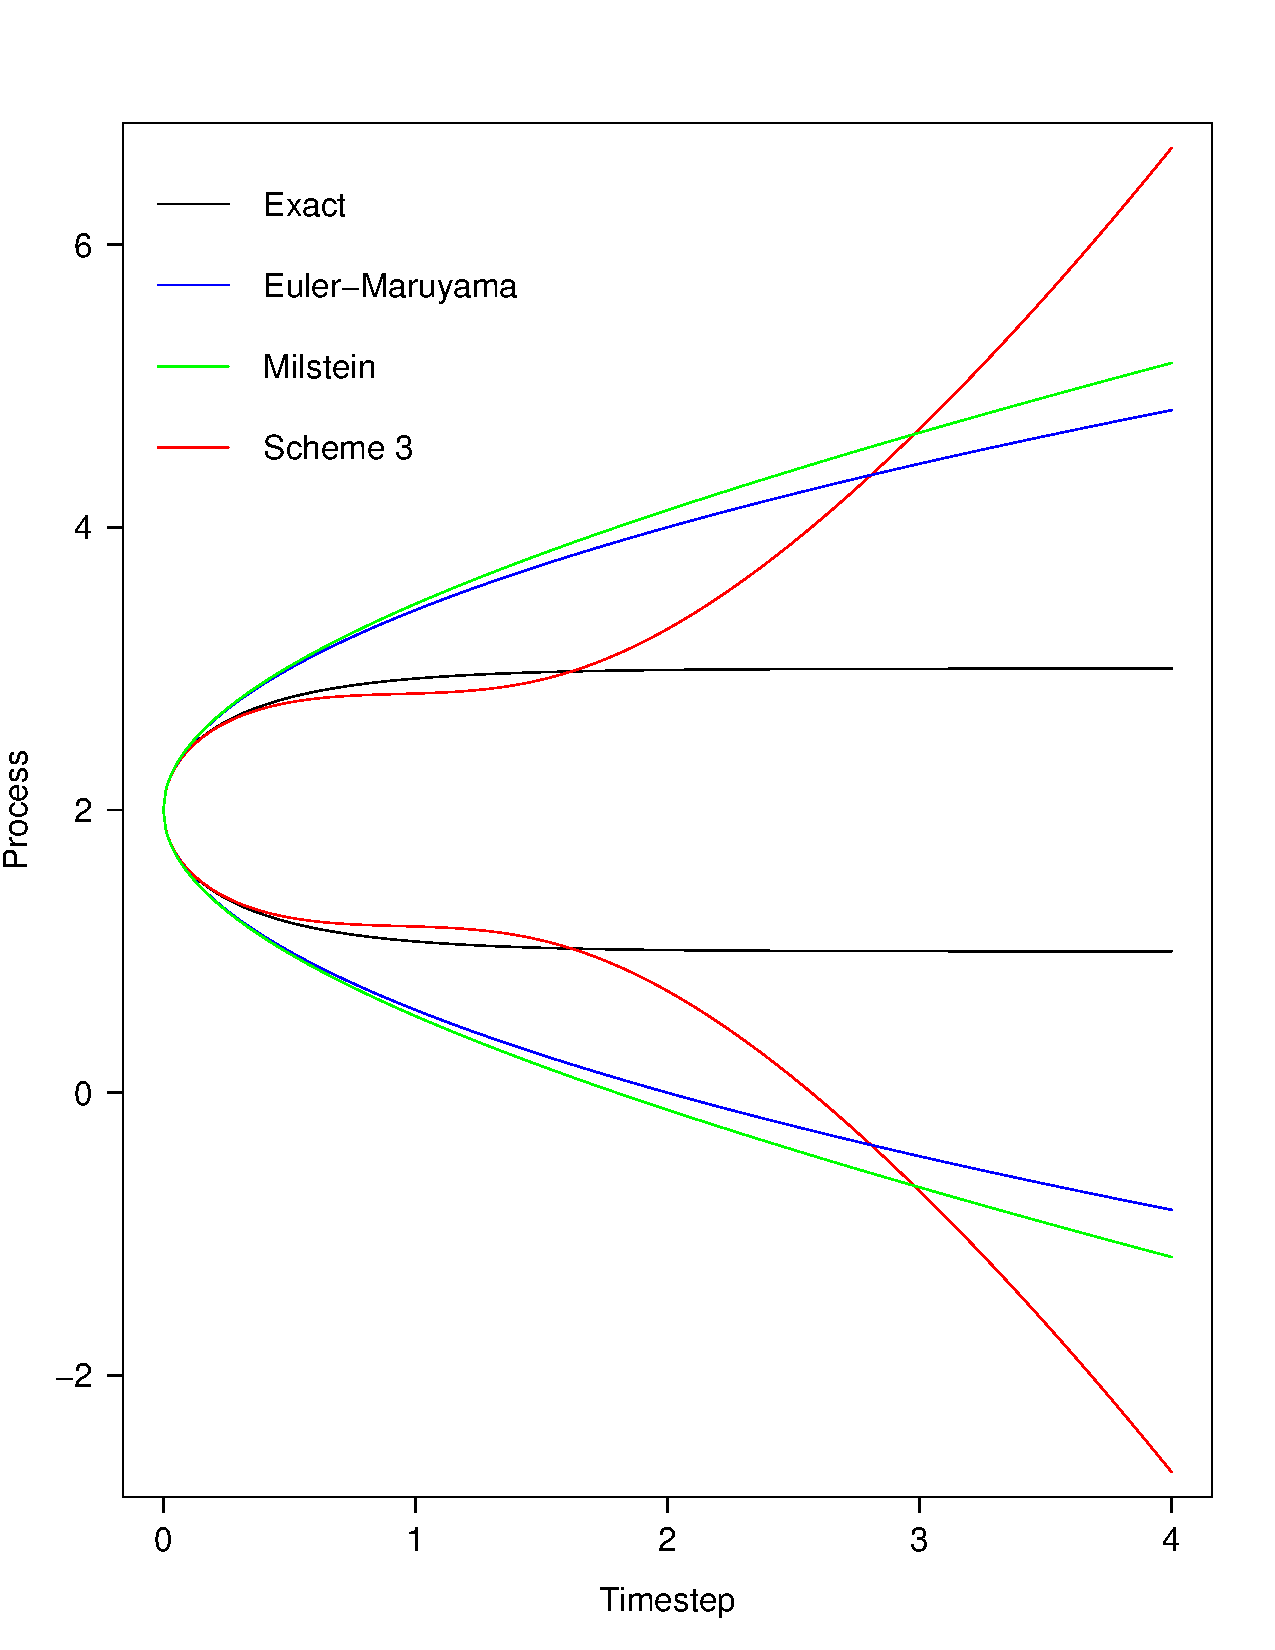
\includegraphics[width=13cm,height=10cm]{./Figures/discretizationError.pdf}
	\rule{35em}{0.5pt}
	\caption[Exact and approximate prediction bands for different discretization schemes]{Exact and approximate prediction bands ($\E[r_t|r_0]\pm SD[r_t|r_0]$) for the CIR process with starting value $r_0=2$ and parameters $\kappa=1$, $\alpha=2$, and $\sigma=1$.}
	\label{fig:discretizationError}
\end{figure}


%\hrule


\subsubsection{Scheme 2: The Milstein Scheme}

The \textit{Milstein Scheme} is slightly more complicated than the Euler-Maruyama scheme and might be regarded as the next step, since it contains one more term from the Itô-Taylor expansions.
It attains strong order of convergence $1.0$ in all cases, not depending on the drift or diffusion coefficients as the Euler-Maruyama scheme.
It reads
\begin{align}\label{Chap4 Sec1.2 Milstein scheme}
X_t=X_{t_0}+\mu I_0 + \sigma I_1 + \sigma\sigma'I_{1,1}.
\end{align}
We see that when the diffusion coefficient is constant, the Milstein scheme reduces to the Euler-Maruyama scheme \eqref{Chap4 Sec1.1 euler scheme}.

\begin{theorem}
	The MGF of the Milstein scheme \eqref{Chap4 Sec1.2 Milstein scheme} is given by the following equation
	\begin{align}
	M_{X_t}(s)=\frac{\exp\left\{ \frac{c_1^2s^2t}{2-4sc_2t} \right\}}{\sqrt{1-2tc_2s}}\exp\left\{ s\left(X_{t_0}+c_3\right) \right\},
	\end{align}
	where 
	\begin{align}\label{Chap4.1.2 Milstein constants}
	c_1=\sigma,\, c_2=\frac{1}{2}\sigma\sigma',\, c_3=\left(\mu-\frac{1}{2}\sigma\sigma'\right)t.
	\end{align}
\end{theorem}
%\begin{proof}
%	To find the MGF, we rearrange the scheme to 
%	\begin{align}\label{Chap4 Sec1.2 Milstein rearangement}
%	X_t-X_{t_0}-c_3 &=c_1J_1+c_2J_1^2,
%	\end{align}
%	where the constants $c_1$, $c_2$, and $c_3$ are as in \eqref{Chap4.1.2 Milstein constants}.
%	We now seek the MGF of the right side of equation \eqref{Chap4 Sec1.2 Milstein rearangement}.
%	Let $Z\sim N(0,t)$, then the MGF of $c_1Z+c_2Z^2$ is defined as
%	\begin{align}
%	M_{c_1Z+c_2Z^2}(s)&=\E\left[e^{(c_1Z+c_2Z^2)s}\right]\notag\\
%	&=\int_{-\infty}^{\infty} e^{\left(c_1z+c_2z^2\right)s} \frac{1}{\sqrt{2\pi t}}e^{-\frac{z^2}{2t}}dz\notag\\
%	&=\frac{1}{\sqrt{2\pi t}}\int_{-\infty}^{\infty} \exp\left\{ -\left(\frac{1}{2t}-c_2 s\right)z^2+c_1sz \right\}dz\notag\\
%	&=\frac{1}{\sqrt{2\pi t}}\int_{-\infty}^{\infty} \exp\left\{ -\left(\frac{1}{2t}-c_2 s\right)(z-q)^2+ \frac{c_1^2s^2t}{2(1-2sc_2t)}\right\}dz\notag\\
%	&=\exp\left\{ \frac{c_1^2s^2t}{2-4sc_2t} \right\}\frac{1}{\sqrt{2\pi t}}\int_{-\infty}^{\infty} \exp\left\{ -\frac{(z-q)^2}{2t(1-2tc_2s)^{-1}} \right\}dz\notag\\
%	&=\frac{\exp\left\{ \frac{c_1^2s^2t}{2-4sc_2t} \right\}}{\sqrt{1-2tc_2s}}\frac{1}{\sqrt{2\pi t}}\frac{1}{(1-2tc_2s)^{-\frac{1}{2}}}
%	\int_{-\infty}^{\infty} \exp\left\{ -\frac{(z-q)^2}{2t(1-2tc_2s)^{-1}} \right\}dz\notag\\
%	&=\frac{\exp\left\{ \frac{c_1^2s^2t}{2-4sc_2t} \right\}}{\sqrt{1-2tc_2s}},
%	\end{align}
%	where $q=c_1st/(1-2sc_2t)$. 
%	The desired MGF is then found by multiplying the MGF for the right hand side and the MGF of $X_{t_0}+c_3$.
%\end{proof}

%\hrule


\subsubsection{Scheme 3: The Itô-Taylor Scheme of Strong Order 1.5}\label{Chap4 Sec1.3 Order 1.5 scheme}
A scheme that can attain strong order 1.5, found in \citet{preston2012approximation} reads
\begin{align}
X_t&=X_{t_0}+\mu I_0 + \sigma I_1 + \sigma\sigma'I_{1,1}\notag\\ 
&+\left(\mu\mu'+\frac{1}{2}\sigma^2\mu''\right)I_{0,0}+\left(\mu\sigma'+\frac{1}{2}\sigma^2\sigma''\right)I_{0,1}
+\sigma\mu'I_{1,0},
\end{align}
or, in a different form:
\begin{align}
X_t-X_{t_0}-c_4&=c_1J_1+c_2J_1^2+c_3J_2,
\end{align}
where
\begin{align}
c_1&=\sigma+\left(\mu\sigma'+\frac{1}{2}\sigma^2\sigma''\right)t,\notag\\
c_2&=\frac{1}{2}\sigma \sigma',\notag\\
c_3&=\sigma\mu'-\mu\sigma'-\frac{1}{2}\sigma^2\sigma'',\notag\\
c_4&=\left( \mu-\frac{1}{2}\sigma\sigma' \right)t+\left(\mu\mu'+\frac{1}{2}\sigma^2\mu''\right)\frac{1}{2}t^2.
\end{align}
\citep{preston2012approximation}

\citet{preston2012approximation} then finds the MGF to be
\begin{align}
M_{X_t}(s)=\frac{\exp\left\{ \frac{\left(6c_1^2+6c_1c_3t+2c_3^2t^2-c_3^2t^3sc_2\right)ts^2}{12-24sc_2t} \right\}}{\sqrt{1-2tc_2s}}\exp\left\{ s\left(X_{t_0}+c_4\right) \right\}.
\end{align}

We note that when the diffusion coefficient $\sigma(t,X_t)$ is constant, this scheme is Gaussian, having mean 
$\mu t+\left(\mu\mu'+\frac{1}{2}\sigma^2\mu''\right)\frac{1}{2}t^2$ and variance
$\left( \sigma^2+\sigma^2\mu't+\frac{1}{3}(\sigma\mu't)^2 \right)t$. It will then have strong order of convergence 1.5, but in the case of a nonconstant diffusion term, it has strong order of convergence 1.0.














%\subsection{maybeadd rewrite}
%
%The approximation schemes in \citet{preston2012approximation} are based on an iterative application of Itô calculus' version of the chain rule, Itô's lemma (see e.g. \citet{oksendal2003stochastic}).
%This iterative application leads to the \textit{Itô-Taylor expansions}, similar to ordinary Taylor expansions.
%For an in-depth study of the Itô-Taylor expansions and their use, we refer to \citet{kloeden1992numerical}, from which the material in the following section is taken.
%For completeness, we revisit the argument here.
%\begin{lemma}
%	Consider a stochastic process defined by $Y_t=f(t,X_t)$ where $X_t$ is governed by the SDE in \ref{integral_ito}.
%	 Then $Y_t$ is defined by:
%	\begin{align}
%	Y_t&=Y_{t_0}+\int_{t_0}^{t}L^0f(s,X_s)ds+\int_{t_0}^{t}L^1f(s,X_s)dW_s,
%	\end{align}
%	where the operators $L^0$ and $L^1$ are defined by
%	\begin{align}
%	L^0&=\frac{\partial}{\partial t}
%	+\mu\frac{\partial}{\partial x}+\frac{1}{2}\sigma^2\frac{\partial^2}{dx^2},\\
%	L^1&=\sigma\frac{\partial}{\partial x}.
%	\end{align} 
%\end{lemma}
%The Itô-Taylor expansions are then obtained by repeatedly applying Itô's lemma to the integrands.
%To outlign the expansions after the first couple of applications, we first let $I_{i_1,i_2,...,i_k}$ represent the multiple It\^o integral, defined as
%\[  I_\alpha = \left\{
%\begin{array}{ll}\label{Chap2 Sec2.1 multiple ito}
%1 & \text{if } k=0, \\
%\int_{t_0}^{t}I_{\alpha^-} ds & \text{if } k\geq 1 \text{ and } \alpha_k=0,\\
%\int_{t_0}^{t}I_{\alpha^-} dW_s & \text{if } k\geq 1 \text{ and } \alpha_k= 1,\\
%\end{array} 
%\right. \]
%where $\alpha = (\alpha_1,\alpha_2,...,\alpha_k)^T$ is a $k$-dimensional vector of zeros and ones, and  $\alpha^-$ denotes the multi-index that can be obtained by deleting the last component of $\alpha$. For example,
%\begin{align}
%I_{0,1,0}=\int_{0}^{t}I_{0,1} ds_1 = \int_{0}^{t}\int_0^{s_1}I_{0}   ds_2ds_1    =\int_{0}^{t}\int_0^{s_1}\int_0^{s_2}ds_3dW_{s_2}ds_1.
%\end{align}
%The acquired Itô-Taylor expansion where $R$ only contains quadruple or higher integrals reads:
%\begin{align}
%X_t&=X_{t_0}+\mu(t_0,X_{t_0})I_0+\sigma(t_0,X_{t_0})I_1\notag\\
%&+L^0\mu(t_0,X_{t_0})I_{0,0}+L^1\mu(t_0,X_{t_0})I_{1,0}\notag\\
%&+L^0\sigma(t_0,X_{t_0})I_{0,1}+L^1\sigma(t_0,X_{t_0})I_{1,1}\notag\\
%&+L^0L^0\mu(t_0,X_{t_0})I_{0,0,0}+L^1L^0\mu(t_0,X_{t_0})I_{1,0,0}\notag\\
%&+L^0L^1\mu(t_0,X_{t_0})I_{0,1,0}+L^1L^1\mu(t_0,X_{t_0})I_{1,1,0}\notag\\
%&+L^0L^0\sigma(t_0,X_{t_0})I_{0,0,1}+L^1L^0\sigma(t_0,X_{t_0})I_{1,0,1}\notag\\
%&+L^0L^1\sigma(t_0,X_{t_0})I_{0,1,1} + L^1L^1\sigma(t_0,X_{t_0})I_{1,1,1}+R.
%\end{align}
%
%It is then possible to construct schemes by neglecting the remainder.
%The \textit{Euler-Maruyama scheme} $\euler$ that approximates $X_t$ consists of the following terms:
%\begin{align}\label{Euler maruyama scheme}
%\euler = X_{t_0}+\mu(t_0,X_{t_0})I_0+\sigma(t_0,X_{t_0})I_1.
%\end{align}
%The \textit{Milstein scheme} $\milstein$ that approximates $X_t$ consists of one more term than the Euler scheme:
%\begin{align}\label{Milstein scheme}
%\milstein = X_{t_0}+\mu(t_0,X_{t_0})I_0+\sigma(t_0,X_{t_0})I_1+L^1\sigma(t_0,X_{t_0})I_{1,1}.
%\end{align}
%Our third and most accurate scheme $\schemethree$ consists of all the terms such that the remainder only holds triple or higher integrals:
%\begin{align}\label{scheme 3}
%\schemethree &= X_{t_0}+\mu(t_0,X_{t_0})I_0+\sigma(t_0,X_{t_0})I_1\notag\\
%&+L^0\mu(t_0,X_{t_0})I_{0,0}+L^1\mu(t_0,X_{t_0})I_{1,0}\notag\\
%&+L^0\sigma(t_0,X_{t_0})I_{0,1}+L^1\sigma(t_0,X_{t_0})I_{1,1}.
%\end{align}
%The MGFs of these schemes can be found in \citet{preston2012approximation}, the characteristic function then follows as the MGF evaluated at $is$, i.e. $\phi_X(s)=M_x(s)$.
%Measures on the accuracy of Itô-Taylor expansions are discussed in \citet{kloeden1992numerical}, for such schemes \textit{strong order of convergence} makes sense:
%\begin{definition}[strong order of convergence]
%	We say that a time discrete approximation $X^\delta$ converges strongly with order $\gamma>0$ at time $t$ if there exists a positive constant $C$, not depending on $\delta$ so that
%	\begin{align}
%	\epsilon(\delta) = \E\left[ \left\| X_t - X^\delta(t) \right\|   \right] \leq C\delta\gamma.
%	\end{align}
%	\citep{kloeden1992numerical}
%\end{definition}
%The Euler-Maruyama scheme \ref{Euler maruyama scheme} attains strong order of convergence $0.5$, but can attain the order $1.0$ if the diffusion part is constant.
%The Milstein scheme \ref{Milstein scheme} always attains strong order of convergence 1.0. Note that if the diffusion part is constant it reduces to the Euler scheme.
%Scheme three can attain strong order of convergence 1.5 if the diffusion part is constant, otherwise it attains strong order 1.0. \citep{kloeden1992numerical, preston2012approximation}
%
%
%%\hrule
%%\mbox{}
%%\vspace{1cm}




\section{Approximating the inverse Fourier transform}
\label{sec::ift}

Consider the case where one has time series data generated by a stochastic process. % from a time series observed at discrete time points, and one a model of the time series.
For likelihood-based inference, one needs the transition density to build the likelihood function.
But this transition density is not always readily available from the model.
This chapter considers the instances where the \textit{characteristic function}, the \textit{moment generating function} (MGF), or the \textit{cumulative generating function} (CGF) of the one step transition is available, but not the transition density.
By definition, the transition density is the \textit{inverse Fourier transform} (IFT) of the characteristic function.
This transformation can be approximated by the \textit{discrete Fourier transform} (DFT). 
Another possible solution is to estimate the transition density with a saddlepoint approximation (SPA), which is derived from the MGF or the CGF.
In this chapter we discuss these two approximations of the IFT, to obtain the transition density.
%In this chapter we state the definition of 
%We will in this chapter derive the SPA, and then proceed to discuss such properties as the need for renormalization, and for what instances an approximation of that kind is beneficial.
%\hrule
%\mbox{}
%\vspace{1cm}

\subsection{The Fourier Transform}
\label{Sec: fourier transform}
%For our purpose, we consider the Fourier transf
The Fourier transform has applications to a large variety of research such as signal analysis, quantum physics, and probability theory.
It relates to probability theory since the characteristic function and the probability density function of a random variable form a Fourier pair.
The definition of a Fourier pair is as follows \citep{kleppe2006numerical}:
\begin{definition}\label{def: fourier transform}
	Consider the function $f$ on $[-\infty,\infty]$. %the interval $S=[-A,A]$ where $A\in(0,\infty]$.
	The \textit{Fourier transform} of $f$ is the function $\hat{f}$ such that
	\begin{align}
	\hat{f}(s) &= \int_{-\infty}^\infty f(x)e^{isx}dx.
	\end{align}
	Conversely, we say that $f$ is the \textit{inverse Fourier transform } of $\hat{f}$ and satisfy
	\begin{align}
	f(x) &= \frac{1}{2\pi}\int_{-\infty}^\infty \hat{f}(s)e^{-isx} ds.
	\end{align}
	We say that the functions $f$ and $\hat{f}$ form a \textit{Fourier pair}.
\end{definition}
%It can be shown that the Fourier transform is a continuous operator $F:L^(R)\to L 
From definition \ref{def: fourier transform} we see that the probability density function and the characteristic function of a random variable $X$ form a Fourier pair if we let $f(x)=0$ when $x$ is outside the probability space of $X$.
We formulate this as a theorem:
\begin{theorem}
	For a random variable $X$, the probability density function $f_X(x)$ 
	and the characteristic function $\phi_X(s)$ of $X$ form a Fourier pair.
	%The interval $S$ is then the support of $f_X(x)$.
\end{theorem}
\begin{proof}
	\begin{align}
	\phi_X(s)=\E\left[e^{isX}\right]=\int_{-\infty}^\infty e^{isx}f_X(x)dx = \hat{f}_X.
	\end{align}
\end{proof}
In this article, we work with random variables for which the probability density is unknown in closed form, but where the characteristic function (or at least an approximation) is.
The inverse Fourier transform then has to be approximated numerically.
For such instances, the following lemma comes in handy.
\begin{lemma}\label{lemma: characteristic conjugate}
	The characteristic function is conjugate symmetric \citep{kleppe2006numerical}:
	\begin{align}
	\phi_X(s) = \overline{\phi_X(-s)}.
	\end{align}
\end{lemma}
%\begin{proof}
%	From the definition of the characteristic function, we have:
%	\begin{align}
%	\phi_X(s) &= \int_{-\infty}^{\infty}f_X(x)e^{ix s} dx\notag\\
%	&=\int_{-\infty}^{\infty}f_X(x)cos(ix s)dx 
%	+ i \int_{-\infty}^{\infty} f_X(x)sin(ix s)dx   \notag \\
%	&=\int_{-\infty}^{\infty} f_X(x) cos(-ix s)dx - i \int_{-\infty}^{\infty}f_X(x)sin(-ix s)dx\notag \\
%	&=\overline{\int_{-\infty}^{\infty} f_X(x)e^{-ix s}dx}\notag\\
%	&=\overline{\phi_X(-s)}.
%	\end{align}
%\end{proof}
The usefulness of lemma \ref{lemma: characteristic conjugate} is due to the fact that, the probability density being a real valued function, the integral can be simplified:
\begin{theorem}\label{theorem: IFT simplified}
	%Let $A$ be the largest positive value in the support of $f_X$, then 
	The inverse Fourier transform of the characteristic function can be simplified as follows:
	\begin{align}
	f_X(x)=\frac{1}{\pi}\int_0^\infty \cRe \left(\phi_X(s)e^{-isx}\right) ds.
	\end{align}
\end{theorem}
%\begin{proof}
%	Since the probability density function is real, it holds that
%	\begin{align}
%	f_X(x) = \frac{1}{2\pi} \int_{-\infty}^\infty \Re\left(\phi_X(s)e^{-isx}\right) ds.
%	\end{align}
%	Now, by investigating the integrand, we have by lemma \ref{lemma: characteristic conjugate}:
%	\begin{align}
%	\Re\left\{ \phi_X(s)e^{-isx}   \right\}&=
%	\Re\left\{ \overline{ \phi_X(s)e^{-isx}}  \right\}
%	= \Re\left\{ \overline{ \phi_X(s)}\overline{e^{-isx}}  \right\}
%	=\Re\left\{ \phi_X(-s)e^{isx}   \right\},
%	\end{align}
%	which means that the real part of the original integrand is symmetric, implying
%	\begin{align}
%	f_X(x)=\frac{1}{\pi}\int_0^\infty \Re \left(\phi_X(s)e^{-isx}\right) ds.
%	\end{align}
%\end{proof}
As noted earlier, the Fourier transform often has to be approximated.
This can be done by the efficient \textit{fast forward Fourier transform} (FFT) algorithm, which utilizes properties such as the one discussed above.
For the instances where we do not have the probability density function readily available, we estimate it using the FFT algorithm already implemented in R, and use this as our benchmark instead of the exact.
In chapter \ref{Chapter6} we shall use our own algorithm that approximates the IFT directly with Gauss-Laguerre quadrature, also making use of theorem \ref{theorem: IFT simplified}.


\subsection{Derivation of the Saddlepoint Approximation}
\label{Chap3.2}

%Having developed the Laplace Approximation \ref{Chap3.1 laplace}, we now wish to show its connection with the Saddlepoint Approximation (SPA) to a density.
Instead of approximating the IFT directly, there exist approximations that can lead to closed form expressions.
In this article  we consider the \textit{saddlepoint approximation} (SPA) to the density $f_X(x)$.
The SPA is often stated in terms of the mean of i.i.d. random variables, where the SPA is the leading term of an asymptotic expansion (similar to the Laplace approximation) \citep{butler2007saddlepoint}.
We shall, however, limit ourselves to the case of $n=1$, or, in other words, of only one continuous random variable.

\begin{theorem}\label{Chap3.2 SPA th}
	For a continuous random variable $X$ with CGF $K_X$ and unknown density $f_X$, the saddlepoint density approximation to $f_X(x)$ is given by 
	\begin{align}
	\text{spa}\left(f_{X};x\right) = \frac{1}{\sqrt{2\pi K_X''(\hat{s})}}\exp\left\{ K_X(\hat{s})-\hat{s}x  \right\},
	\end{align}
	where $\hat{s}=\hat{s}(x)$ is the \textit{saddlepoint}, that is the unique solution to the equation
	\begin{align}\label{Chap3.2 IP}
	K_X'(\hat{s}) = x,
	\end{align}
	referred to as the \textit{saddlepoint equation} or the \textit{inner problem} \citep{butler2007saddlepoint}.
	
	\begin{proof}
		For a random variable $X$, the \textit{moment generating function} (MGF) $M_X(s)$ is defined as
		\begin{align}
		M_X(s)=\int_{-\infty}^{\infty} e^{sx}f_X(x)dx,
		\end{align}
		where $f_X(x)$ is the probability density function of $X$. By using the Fourier inversion formula, we can obtain the density $f$ from the MGF:
		\begin{align}\label{Chap3.2 fourier inversion int}
		f_X(x)&=\frac{1}{2\pi}\int_{-\infty}^{\infty}M_X(is)\exp\{-isx\} dt\notag\\
		&=\frac{1}{2\pi}\int_{-\infty}^{\infty}\exp\left\{ K_X(is)-isx \right\} ds,
		\end{align}
		%where $K_X(s)$ is the \textit{cumulative generating function} (CGF)
		\citep{goutis1999explaining}.
		
		%The idea is now to show that the Laplace approximation \ref{Chap3.1 laplace} is applicable to this integral, such that
		%\begin{align}
		%	f_X(x)\approx \hat{f}_X(x)=\frac{1}{\sqrt{2\pi K_X''(\hat{s})}}\exp\left\{ K_X(\hat{s})-\hat{s}x  \right\},
		%\end{align}
		%where $\hat{s}$ is the saddlepoint \ref{Chap3.2 IP}. 
		
		First, we apply a change of variable, $u=it$ to the integral \ref{Chap3.2 fourier inversion int}:
		\begin{align}
		f_X(x)= \frac{1}{2\pi i} \int_{-i\infty}^{i\infty}e^{K(u)-ux}du,
		\end{align}
		and note that the value of the integral is unchanged if we integrate through a line parallel to the imaginary axis:
		\begin{align}
		f_X(x)&= \frac{1}{2\pi i} \int_{\tau-i\infty}^{\tau+i\infty}e^{K_X(u)-ux}du\notag\\
		&=\frac{1}{2\pi}\int_{-\infty}^{\infty}e^{K_X(\tau+iv)-(\tau+iv)x}dv.
		\end{align}
		Further, we expand the inner part of the exponential about the point $\tau$, and obtain:
		\begin{align}
		K_X(\tau+iv)-(\tau+iv)x = &K_X(\tau)-\tau x + \left( K_X'(\tau)-x \right)iv
		+\sum_{j\geq 2} \frac{K_X^{(j)}(\tau)(iv)^j}{j!},
		\end{align}
		and by choosing $\tau$ to be the saddlepoint, $\hat{s}$, the second term in the expansion disappears.
		Then, from using the transformation $y=\sqrt{K_X''(\hat{s})}v$, we have for the right hand side
		\begin{align}
		\frac{\exp\left\{ K_X(\hat{s})-\hat{s} x \right\}}{2\pi\sqrt{K_X''(\hat{s})}}\int_{-\infty}^{\infty}
		e^{-\frac{1}{2}y^2+O(y^3)}dy.
		\end{align}
		Neglecting the $O(y^3)$ term, and from noting that the integrand then is the integrand of the standard normal density which we evaluate, we obtain our desired result \eqref{Chap3.2 SPA th}.
	\end{proof}
\end{theorem}

The SPA is a powerful tool to compute accurate approximations to the densities of random variables, but it comes to the cost of computing $\hat{s}(x)$, $K_X(\hat{s}(x),x)$, and $\left.\frac{\partial^2}{\partial s^2}K_X(s,x)\right|_{\hat{s}(x)}$ for each new value of $x$.
In the next section we will look at some of the properties and the drawbacks of the SPA.




%\hrule
%\mbox{}
%\vspace{1cm}



\subsection{Renormalization of the Saddlepoint Approximation}
\label{Chap3.3}

The perhaps most serious problem with the SPA is, that for models deviating from the Gaussian, it does not integrate to 1 (w.r.t. $x$).
Indeed, it is the case that the SPA is  only exact up to a multiplicative constant for the normal, gamma, and inverse Gaussian densities \citep{kolassa2006series}. In applications of the SPA, such as maximum likelihood estimation (MLE), where the model deviates substantially from a Gaussian model, the likelihood estimates with the current SPA will not be accurate enough \citep{kleppe2008building}.
%One way to think of it is that the different probabilities are weighted unequally (depending on how the SPA integrates), leading to biased estimates. (ask Hans if correct way to think of it)\\

One way to deal with this problem is, then, to develop an alternative SPA with non-Gaussian leading terms \citep{kleppe2008building, ai2006saddlepoint}. 
However, in small dimensions it is feasible to do a \textit{renormalization} of the SPA. 
This basically means to multiply the SPA with a constant $c^{-1}$ so that $c$ is the integral of the SPA (w.r.t. $x$) over the whole area. 
%Let $\hat{f}_X(x)$ be the SPA, then 
The renormalized SPA is the function 
\begin{align}\label{Chap3.2 renormalization equation}
\text{rnspa}\left(f_{X};x\right)=\frac{\text{spa}\left(f_{X};x\right)}{\int \text{spa}\left(f_{X};x\right) dx}.
\end{align}
The integral in the denominator usually has to be evaluated numerically. We note that the increase in accuracy comes to the cost of numerically evaluating this integral, bearing in mind the original cost of evaluating the SPA.

%\subsection{Example: Noncentral Chi-Squared}
%\label{Chap3.4}
%
%\begin{figure}[htbp]
%	\centering
%	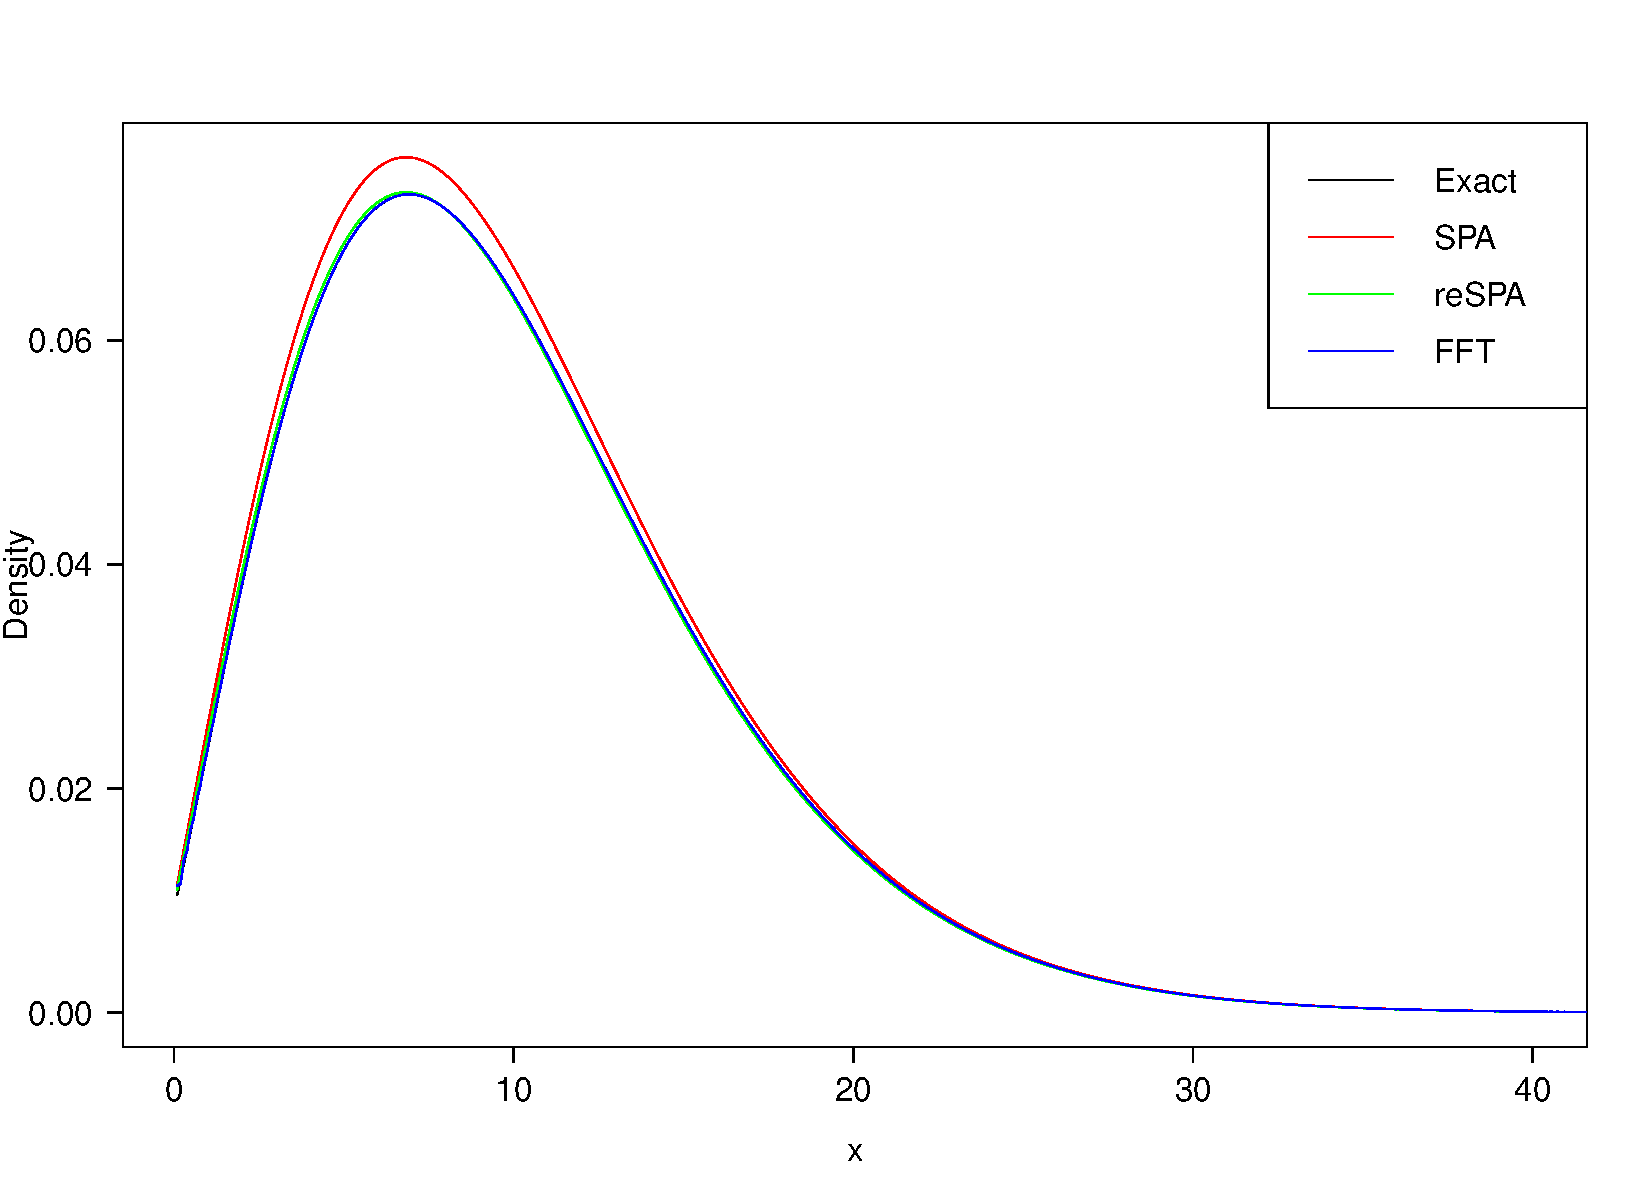
\includegraphics[width=13cm,height=10cm]{./Figures/tdnchisq.pdf}
%	\rule{35em}{0.5pt}
%	\caption[Approximating the inverse Fourier transform: non-central chi-square]{Exact and estimated probability density function for the non-central chi-square distribution for parameters $k=2$ and $\lambda=8$.}
%	\label{fig:nchisq}
%\end{figure}
%
%An interesting application of the SPA, proposed in \citet{goutis1999explaining}, is the \textit{non-central chi-squared} distribution, related to the CIR process \eqref{Chap2.3.3 (CIR)}.
%The probability density function is:
%\begin{align}\label{eq: nchisq poisson mix}
%f_X(x;k,\lambda)=\sum_{i=0}^\infty \frac{x^{k/2+i-1}e^{-x/2}}{\Gamma(k/2+i)2^{k/2+i}}
%\frac{\left(\frac{\lambda}{2}\right)^ie^{-\left(\frac{\lambda}{2}\right)}}{i!},
%\end{align}
%an infinite sum of central chi-squared densities weighted with Poisson probabilities. Another way to write this density, which we will exploit later, is:
%\begin{align}\label{Chap3.3 nchisq density}
%f_X(x;k,\lambda)=\frac{1}{2}e^{-\frac{x+\lambda}{2}}
%\left( \frac{x}{\lambda} \right)^{\frac{k}{4}-\frac{1}{2}} I_{\frac{k}{2}-1}\left(\sqrt{\lambda x}\right),
%\end{align}
%where $I_\nu(x)$ is the modified Bessel function of the first kind. 
%If one does not want to deal with infinite sums, one could exploit that the MGF if quite simple:
%%None of these expressions are easily evaluated, thus the SPA might be used. 
%%It turns out that the MGF of the non-central chi-squared density is quite simple
%\begin{align}
%M_X(t)=\frac{e^{\frac{\lambda t}{1-2t}}}{(1-2t)^\frac{k}{2}}.
%\end{align}
%We solve the saddlepoint equation to obtain
%\begin{align}
%\hat{\tau}=\frac{-k+2x-\sqrt{k^2+4\lambda x}}{4x},
%\end{align}
%which we insert into our expression for the SPA \eqref{Chap3.2 SPA th}. The exact density\footnote{
%	The density plot labelled as the exact density is obtained via the \texttt{dchisq($x,k,\lambda$)} function in R.
%	The R function calculates the density as a Poisson mixture of central chi-squares (approximation of equation \eqref{eq: nchisq poisson mix}), and hence it is not exact \citep{rProject2015}. 
%	However, for our purpose with a small non-centrality parameter, this gives an accurate result which we use as our benchmark and label as exact.
%}
%, the SPA, the renormalized SPA, and the density using the FFT of the characteristic function are plotted in figure \ref{fig:nchisq}.
%We here see that the SPA lies closely to that of the exact density, and this is even more so the case for the renormalized version.
%It is very hard to distinguish the renormalized SPA, the density obtained via the FFT, and the exact density using R from one another by just using the naked eye.
%
%
%
%
%\subsection{Example: Compounded Poisson Process}
%\label{Chap3.5}
%\begin{figure}[htbp]
%	\centering
%	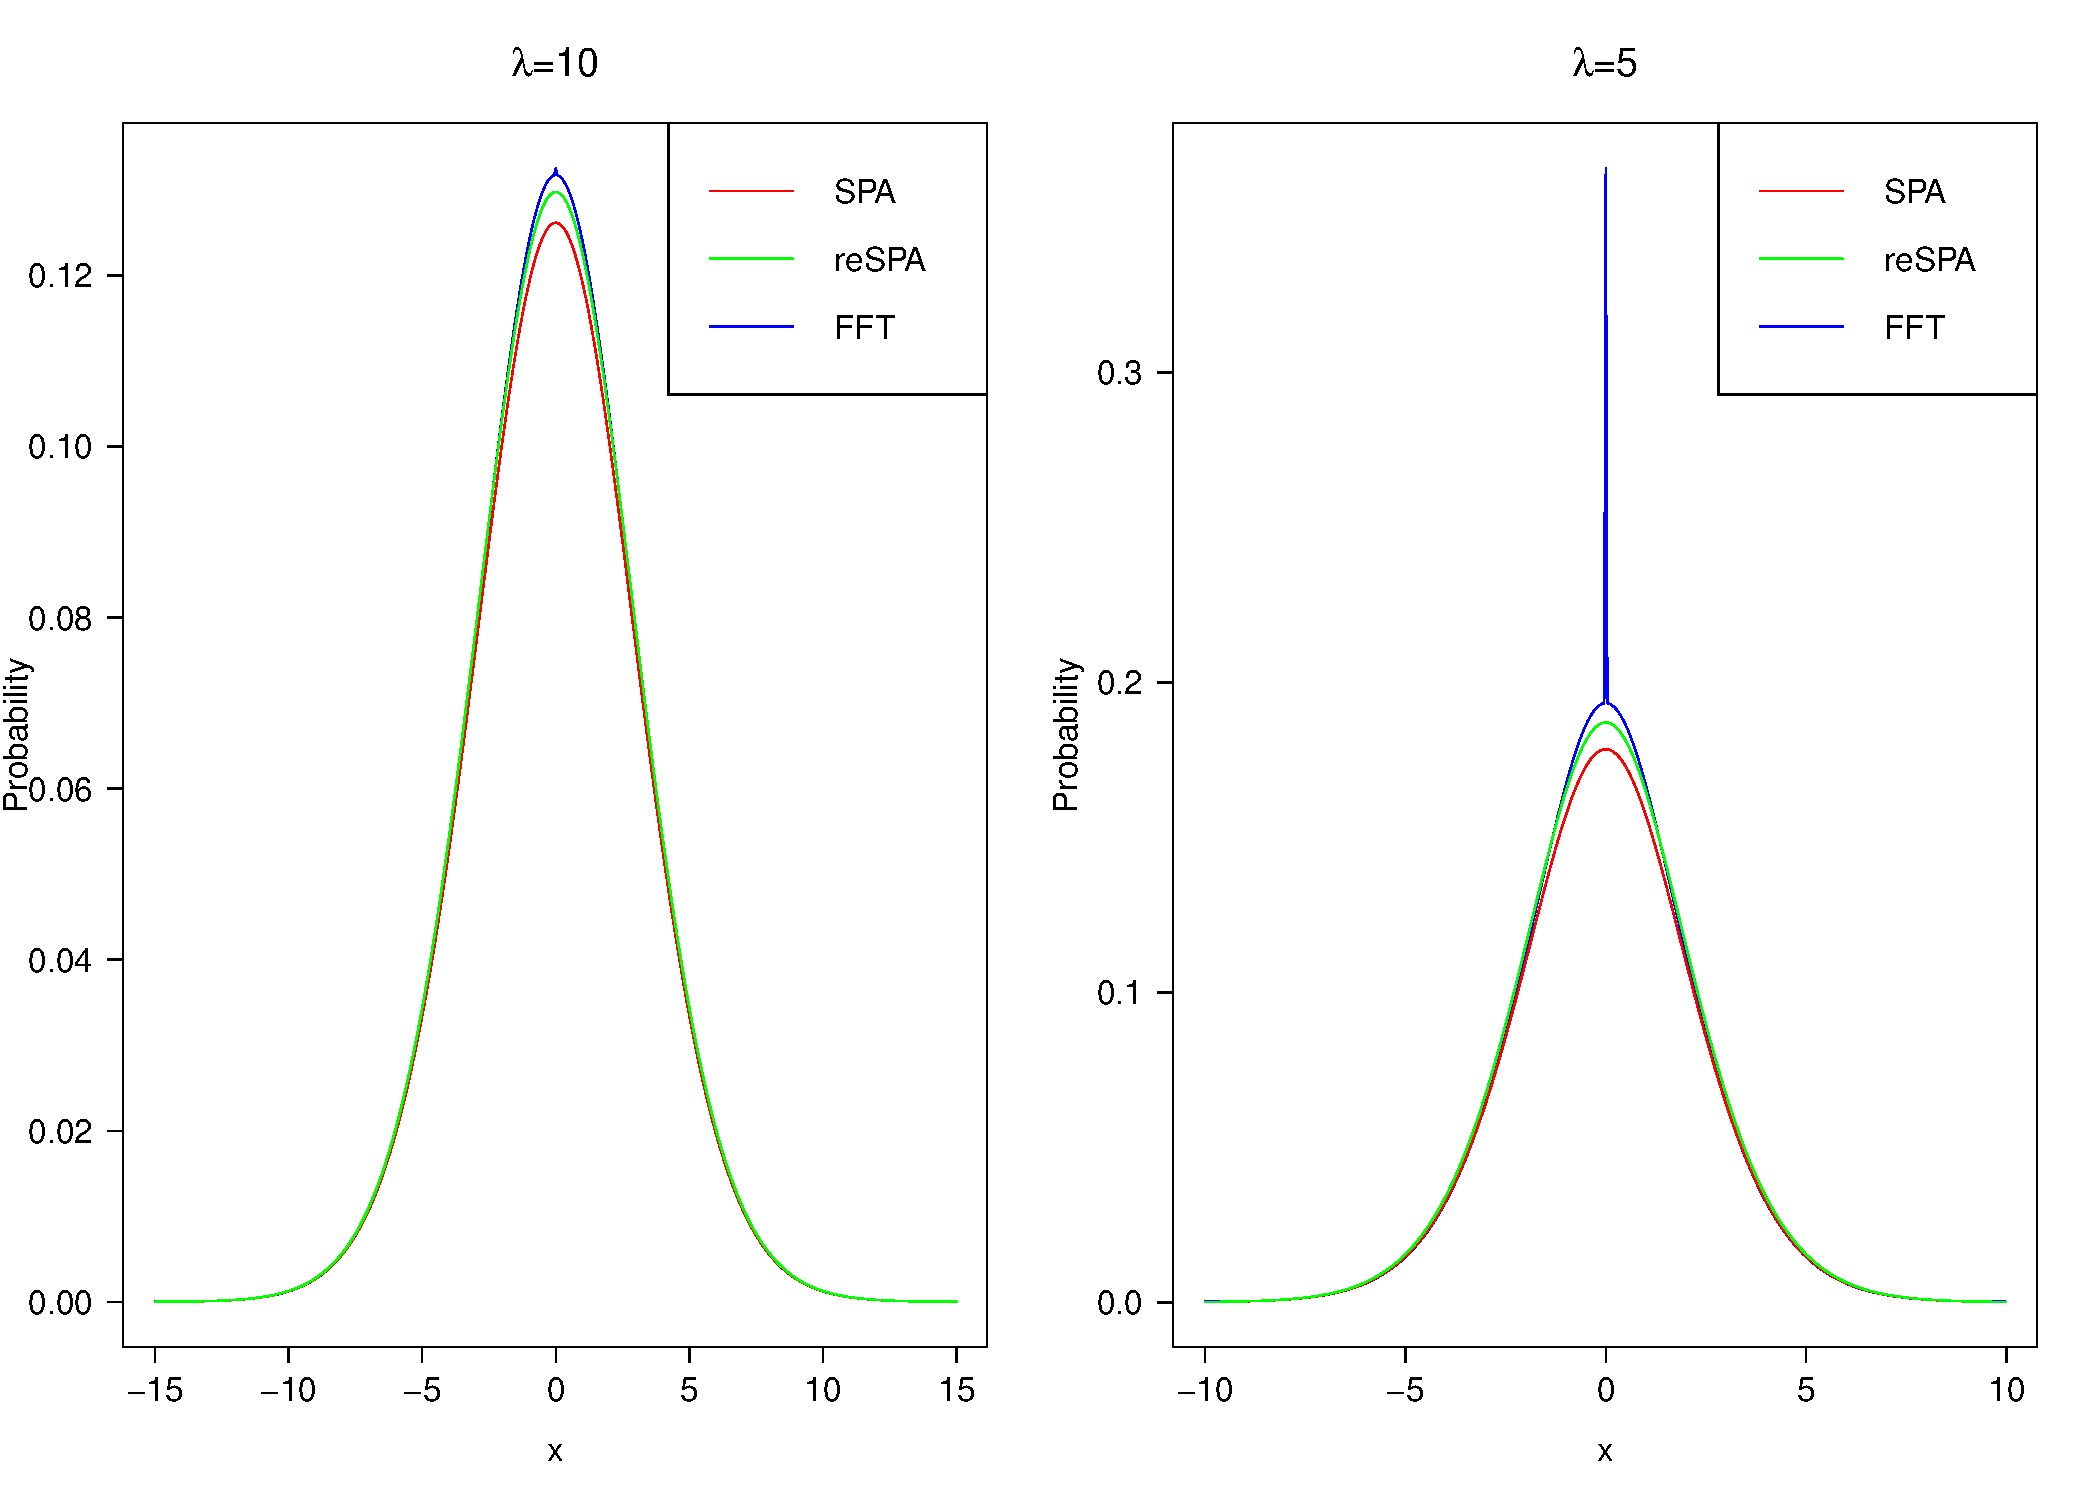
\includegraphics[width=15cm,height=10cm]{./Figures/comPois.pdf}
%	\rule{35em}{0.5pt}
%	\caption[Approximating the inverse Fourier transform: compounded Poisson process]{
%		Exact (FFT) and approximated (SPA and reSPA) transition probabilities for the compounded Poisson process with different values of $\lambda$: $\lambda=10$ and $\lambda=5$.
%		The jumps were standard normal and the time interval was set to $t=1$.
%		%The SPA, the renormalized SPA, empirical density, and histograms are plotted for compounded Poisson processes with different values of $\lambda$. 
%		%Other parameters were fixed with $\mu=0$, $\nu=1$, and $t=1$.
%		%The histograms are plotted for data generated in R, using 100000 simulations for each value of $\lambda$.
%	} \label{fig:cPoisTD}
%\end{figure}
%
%For the previous example, the SPA provides a reasonable approximation of the density, but for different processes this might not be the case.
%One such instance is the compounded Poisson process, defined by equation \eqref{Chap2.2 Def compounded poisson}.
%The CGF can be derived from the MGF \eqref{Chap2.3.4 MGF CP} and reads
%\begin{align}
%K_X(s) =  \lambda t \left( M_Y(s)-1 \right),
%\end{align}
%where $Y$ is the distribution of the iid jumps.
%Taking these to be normally distributed with expectation $\mu$ and variance $\nu^2$, we arrive at:
%\begin{align}
%K_X(s) =  \lambda t \left( e^{s\mu+\frac{1}{2}\nu^2s^2}-1 \right).
%\end{align}
%The inner problem can then be solved using a Newton-type algorithm.
%The SPA and the renormalized SPA are plotted in figure \ref{fig:cPoisTD}, together with the estimated density using the FFT algorithm with the characteristic function. We assume that the latter is reasonably exact.
%
%In figure \ref{fig:cPoisTD} we find that for $\lambda=10$, both the SPA and the renormalized SPA are quite accurate, similar to that of the example with the non-central chi-square distribution.
%As $\lambda$ decreases, they both become more inaccurate at the centre of the density. 
%%Accordingly, a renormalization also becomes more and more necessary.
%An interesting observation concerns the high accuracy of the SPA in the tails.
%In risk management, different risk measures such as \textit{value at risk} and \textit{expected shortfall} (see e.g. \citet[chapter 2.2]{mcneilquantitative}) concern themselves with the behaviour in the tail.
%Since the compounded Poisson process is a popular model especially in insurance for the cumulative amount of claims, but also for other applications such as credit risk \citep{gerhold2010generalization},
%it is conceivable that the SPA might have important applications in this respect.


\subsection{Gaussian quadrature}
Another approach of numerically computing the IFT, is to use numerical integration schemes directly.
Among such integration schemes, the class of Gaussian quadrature rules, especially Gauss-Laguerre and Gauss-Hermite methods, are suitable due to the exponential form of the integrand.

The Gauss-Laguerre method of order $n$ approximates exponentially weighted integrals in the following way \citep{pressnumerical}:
\begin{align}
\int_0^\infty e^{-x}f(x)dx \approx \sum_{i=1}^{n}w_i f(x_i),
\end{align}
where $x_i$ is the i'th root of the Laguerre polynomial of order $n$ defined recursively by
\begin{align}
(i+1)L_{i+1} = (1-x+2i)L_i - iL_{i-1},\,L_0=1,\, L_1 = 1-x,
\end{align}
and $w_i$ are the weights given by
\begin{align}\label{gl-qudrature weights}
w_i = \frac{x_i}{(n+1)^2 \left[L_{n+1}(x_i)\right]^2}.
\end{align}

The Gauss-Hermite method of order $n$ approximates a similar integral:
\begin{align}
\int_0^\infty e^{-x^2}f(x)dx \approx \sum_{i=1}^{n}w_i f(x_i),
\end{align}
where $x_i$ is the i'th root of the Hermite  polynomial of order $n$ defined recursively by
\begin{align}
H_{i+1} = 2xH_i - 2iH_{i-1},\,H_{0}=1,\, H_1 = 2x,
\end{align}
and $w_i$ are the weights given by
\begin{align}\label{gl-qudrature weights}
w_i = \frac{2^{n-1}n!\sqrt{\pi}}
{n^2 \left[H_{n-1}(x_i)\right]^2}.
\end{align}

\subsection{Possibly exact saddlepoint section}



\section{Likelihood estimation}

Likelihood estimation for mixed effect models. 

Proof for compounded Poisson (make general).

Proof for jump diffusion (make general).

Profile likelihood (mjd example)

\section{Numerical results}
\label{sec::numerical_results}

In this section we present numerical results for the methods described in chapter \ref{Chapter4}.
We test the accuracy of the methods by calculating and plotting transition densities, in addition to likelihood-based inference for processes with known solutions and which can be simulated exactly.
The error in the estimated transition densities are measured using the absolute error of the log density.
The processes that are considered are the GBM \eqref{Chap2.3.1 (GBM)}, the OU process \eqref{Chap2.3.2 (OU)}, the CIR process \eqref{Chap2.3.3 (CIR)}, and the MJD model for log returns \eqref{Chap2.3.4 (MJD)}.
The first section considers the transition densities, the second considers likelihood-based analysis.


%In this chapter we will investigate likelihood-based analysis for the the methods described in the previous chapters.
%We will test the methods by calculating the likelihood estimates for benchmark processes with known solutions such as the GBM \eqref{Chap2.3.1 (GBM)}, the OU process \eqref{Chap2.3.2 (OU)}, the CIR process \eqref{Chap2.3.3 (CIR)}, and the MJD model for log returns \eqref{Chap2.3.4 (MJD)}.
%The implementation will be done in \textbf{TMB}, utilizing several nice benefits of this package.
%In section \ref{Chap6.1} we discuss implementation of the joint-negative log-likelihood function in \textbf{TMB} for exact transition densities, the ITSPA, and the renormalized ITSPA.
%Section \ref{Chap6.2} is devoted to numerical results, presented in the form of tables and estimated transition densities over the data.

\subsection{Approximation of Transition Densities}
\label{Chap6 sec: approximation of TD}


%\begin{figure}[htbp]
%	\centering
%	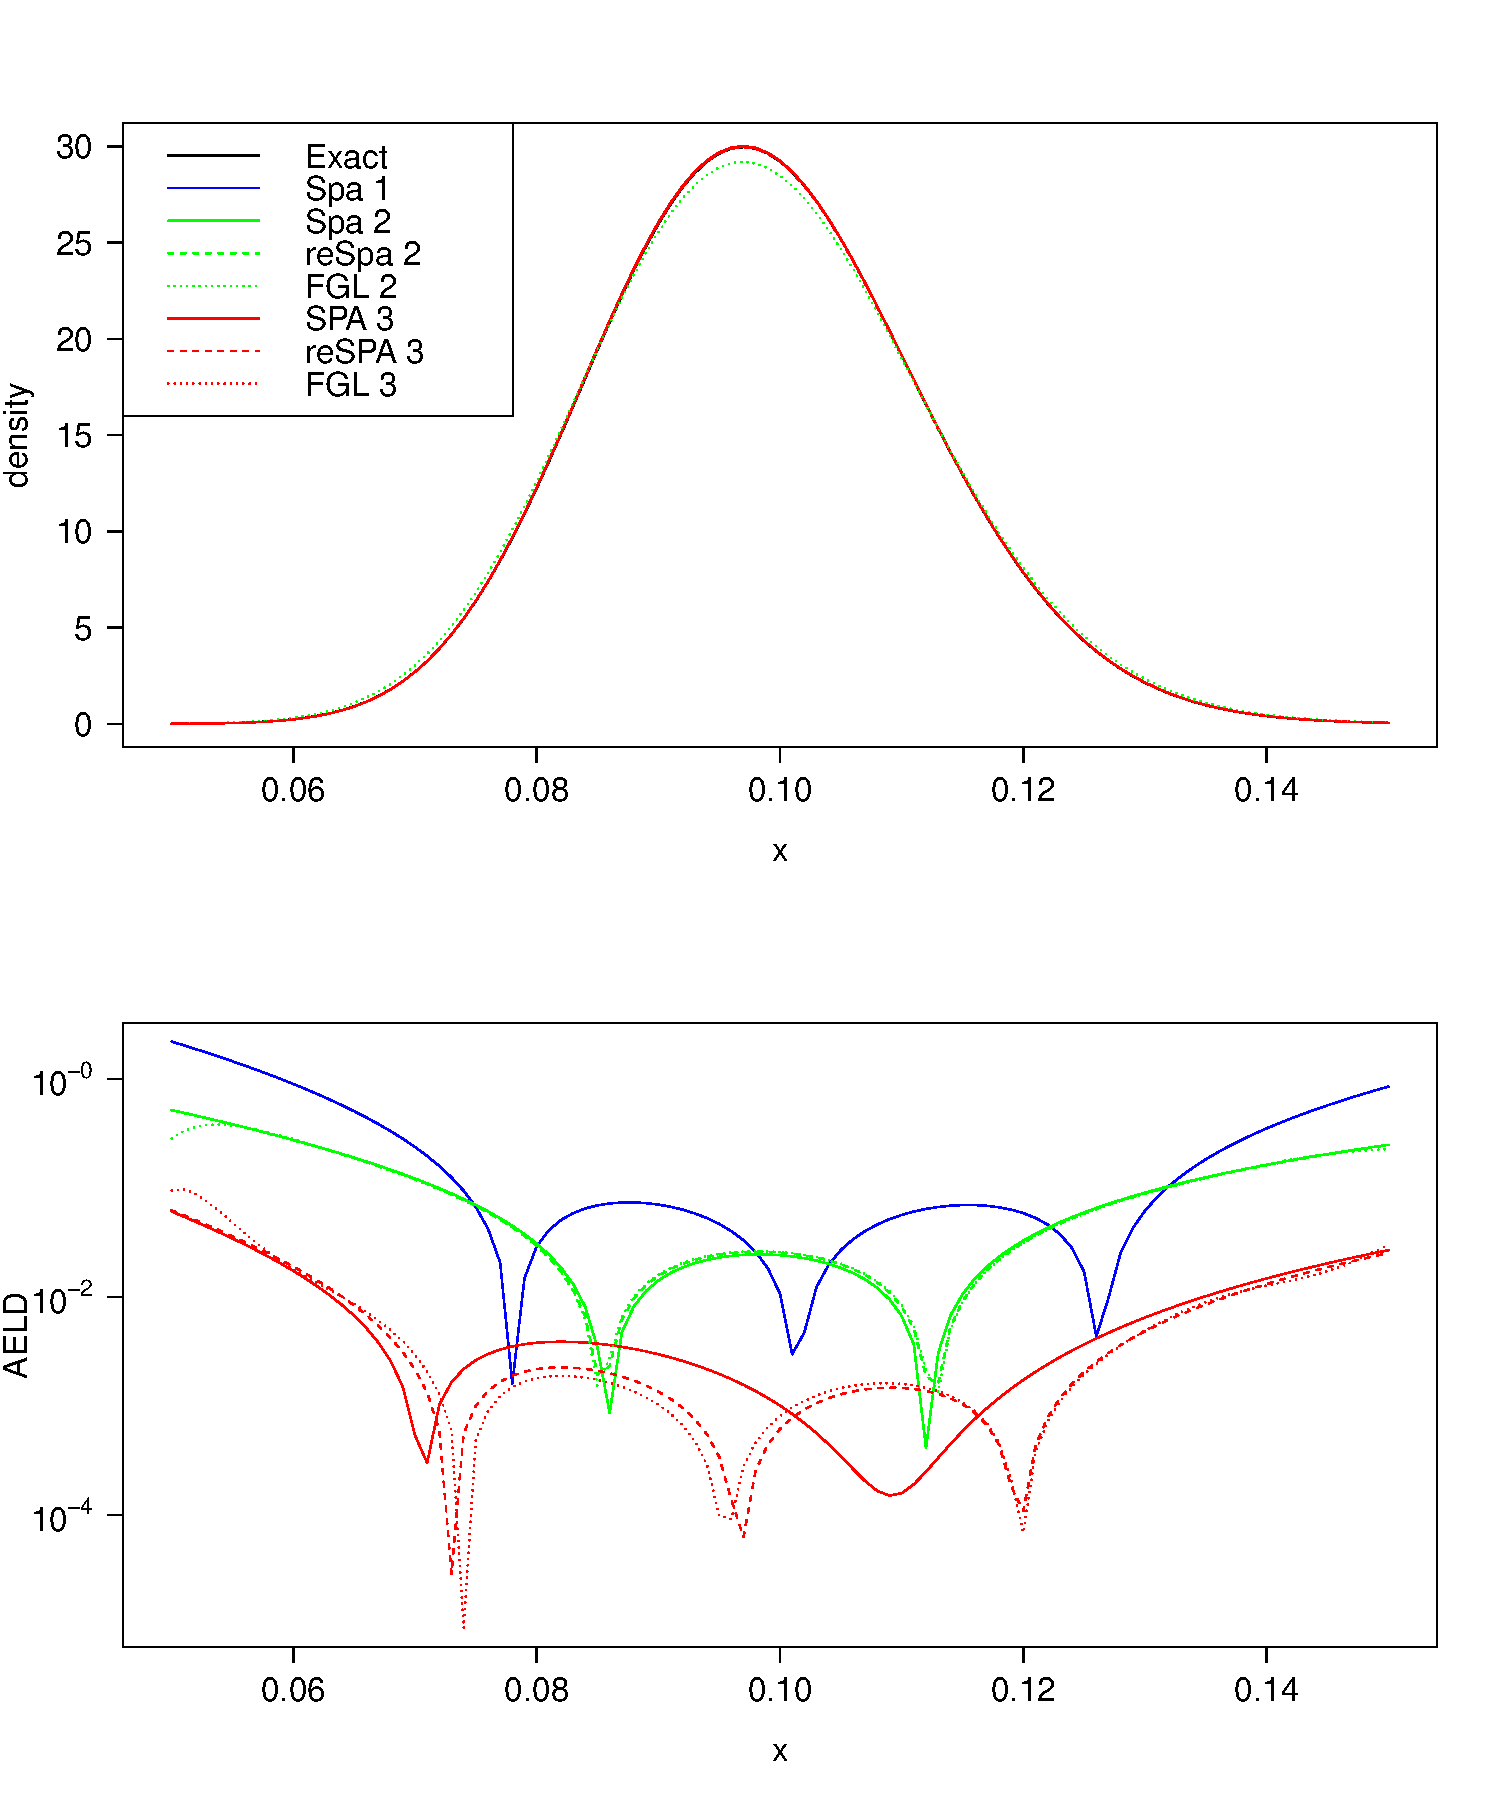
\includegraphics[width=13cm,height=12cm]{./Figures/tdcir1fgl.pdf}
%	\rule{35em}{0.5pt}
%	\caption[Transition densities: Cox-Ingersoll-Ross, small timestep]{(Top) Exact and estimated transition densities for the CIR process with starting value $x_0=0.1$, parameters $\kappa=0.5$, $\alpha=0.06$, and $\sigma=0.15$, and with timestep $t=1/12$.\\
%		(Bottom) AELD plotted for the same values of the estimated transition densities.}\label{fig: tdcir1}
%	\label{fig: tdcir1}
%\end{figure}
%
%\begin{figure}[htbp]
%	\centering
%	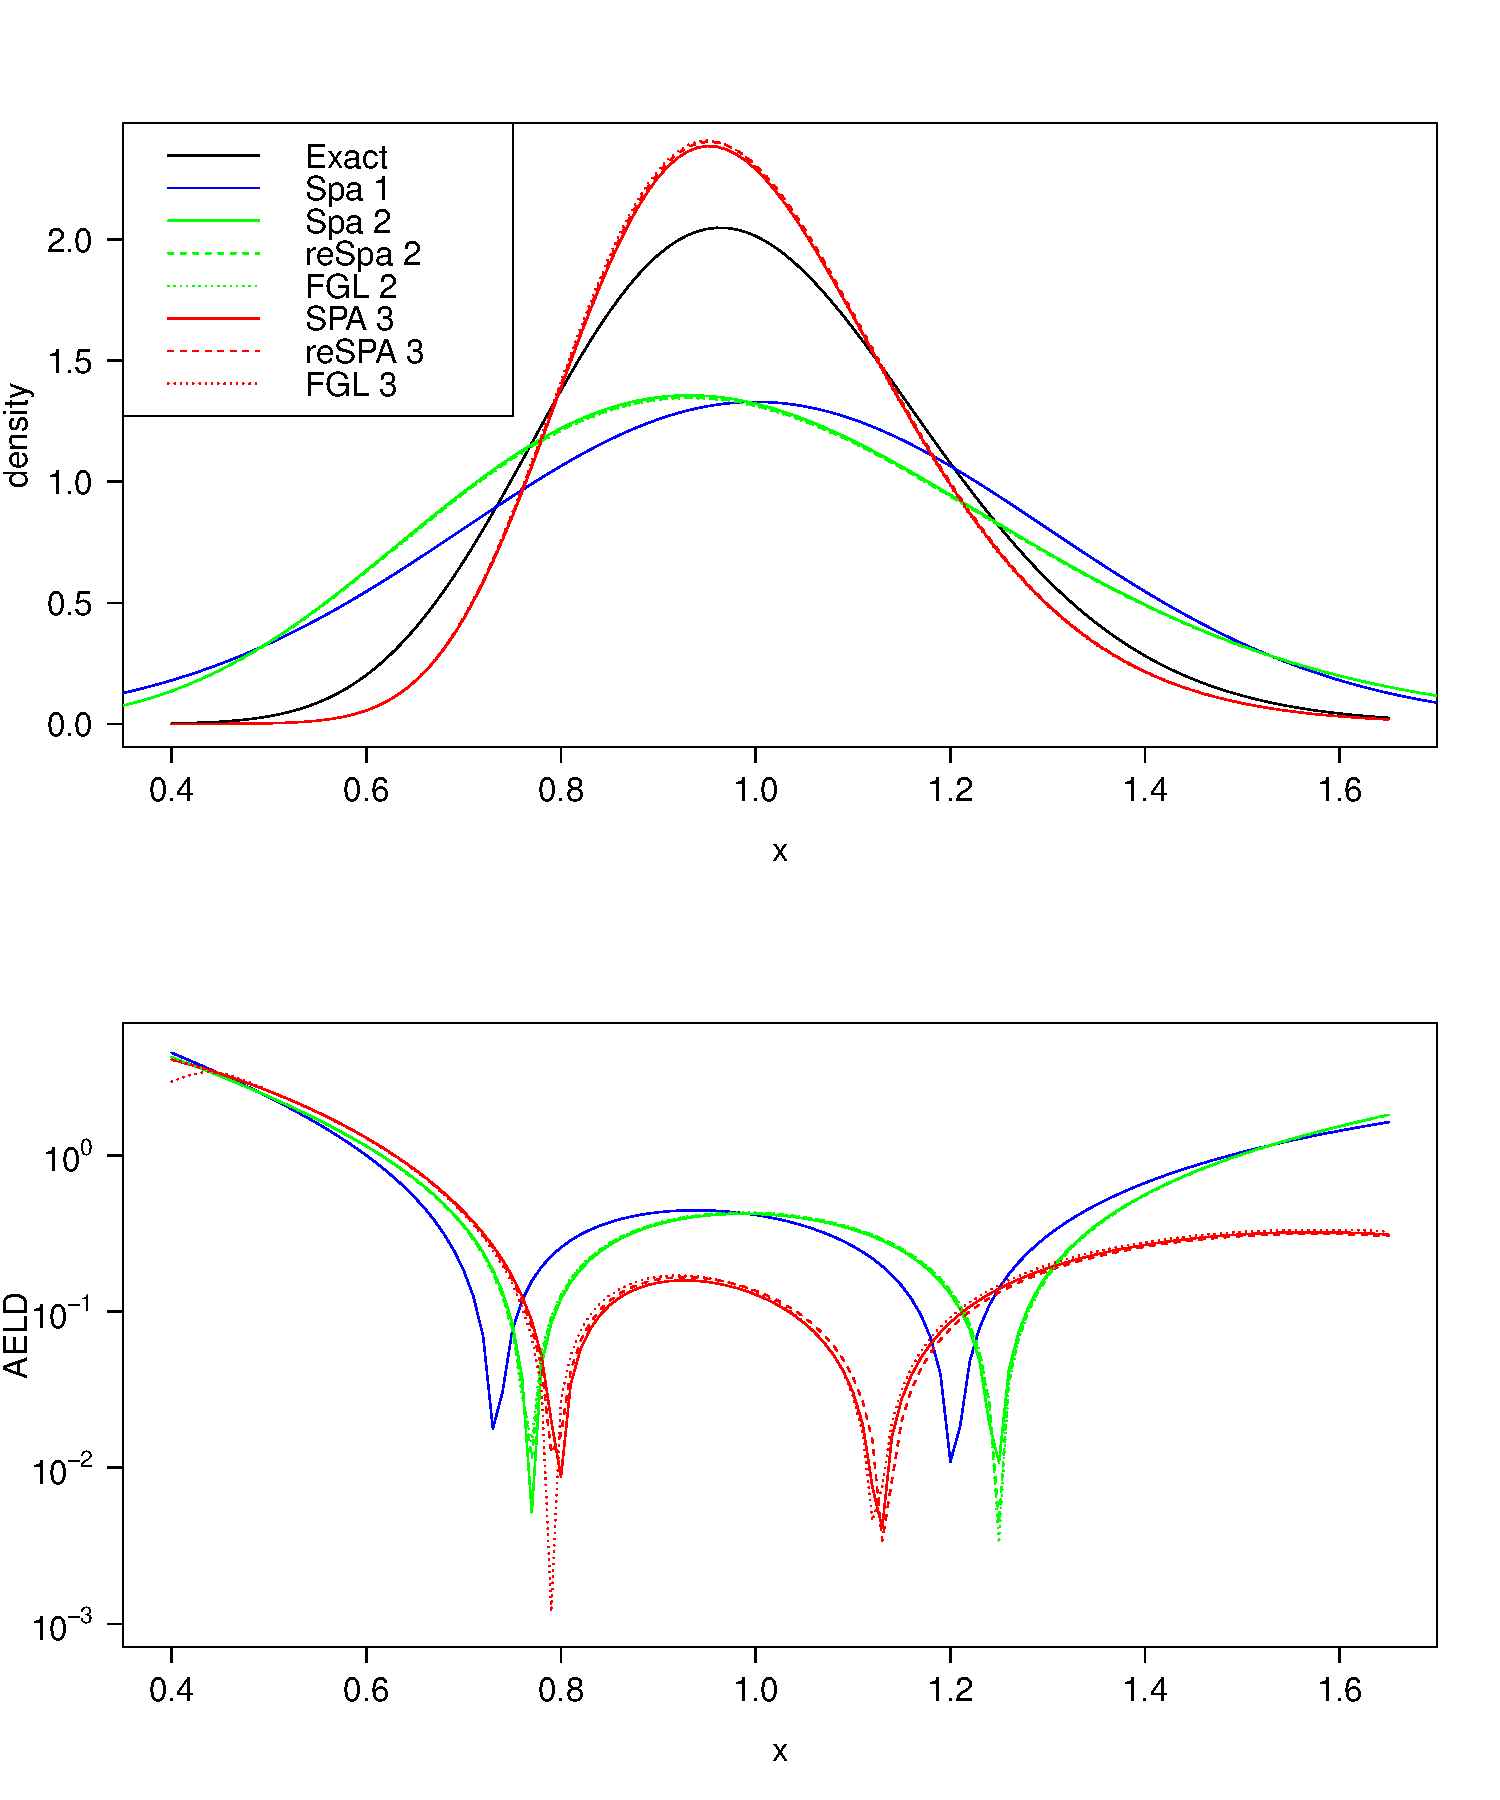
\includegraphics[width=13cm,height=12cm]{./Figures/tdcir2fgl.pdf}
%	\rule{35em}{0.5pt}
%	\caption[Transition densities: Cox-Ingersoll-Ross, large timestep]{(Top) Exact and estimated transition densities for the CIR process with starting value $x_0=1$, parameters $\kappa=1$, $\alpha=1$, and $\sigma=0.3$, and with timestep $t=1$. \\
%		(Bottom) AELD plotted for the same values of the estimated transition densities.}\label{fig: tdcir2}
%	\label{fig: tdcir2}
%\end{figure}

\begin{figure}[htbp]
	\centering
	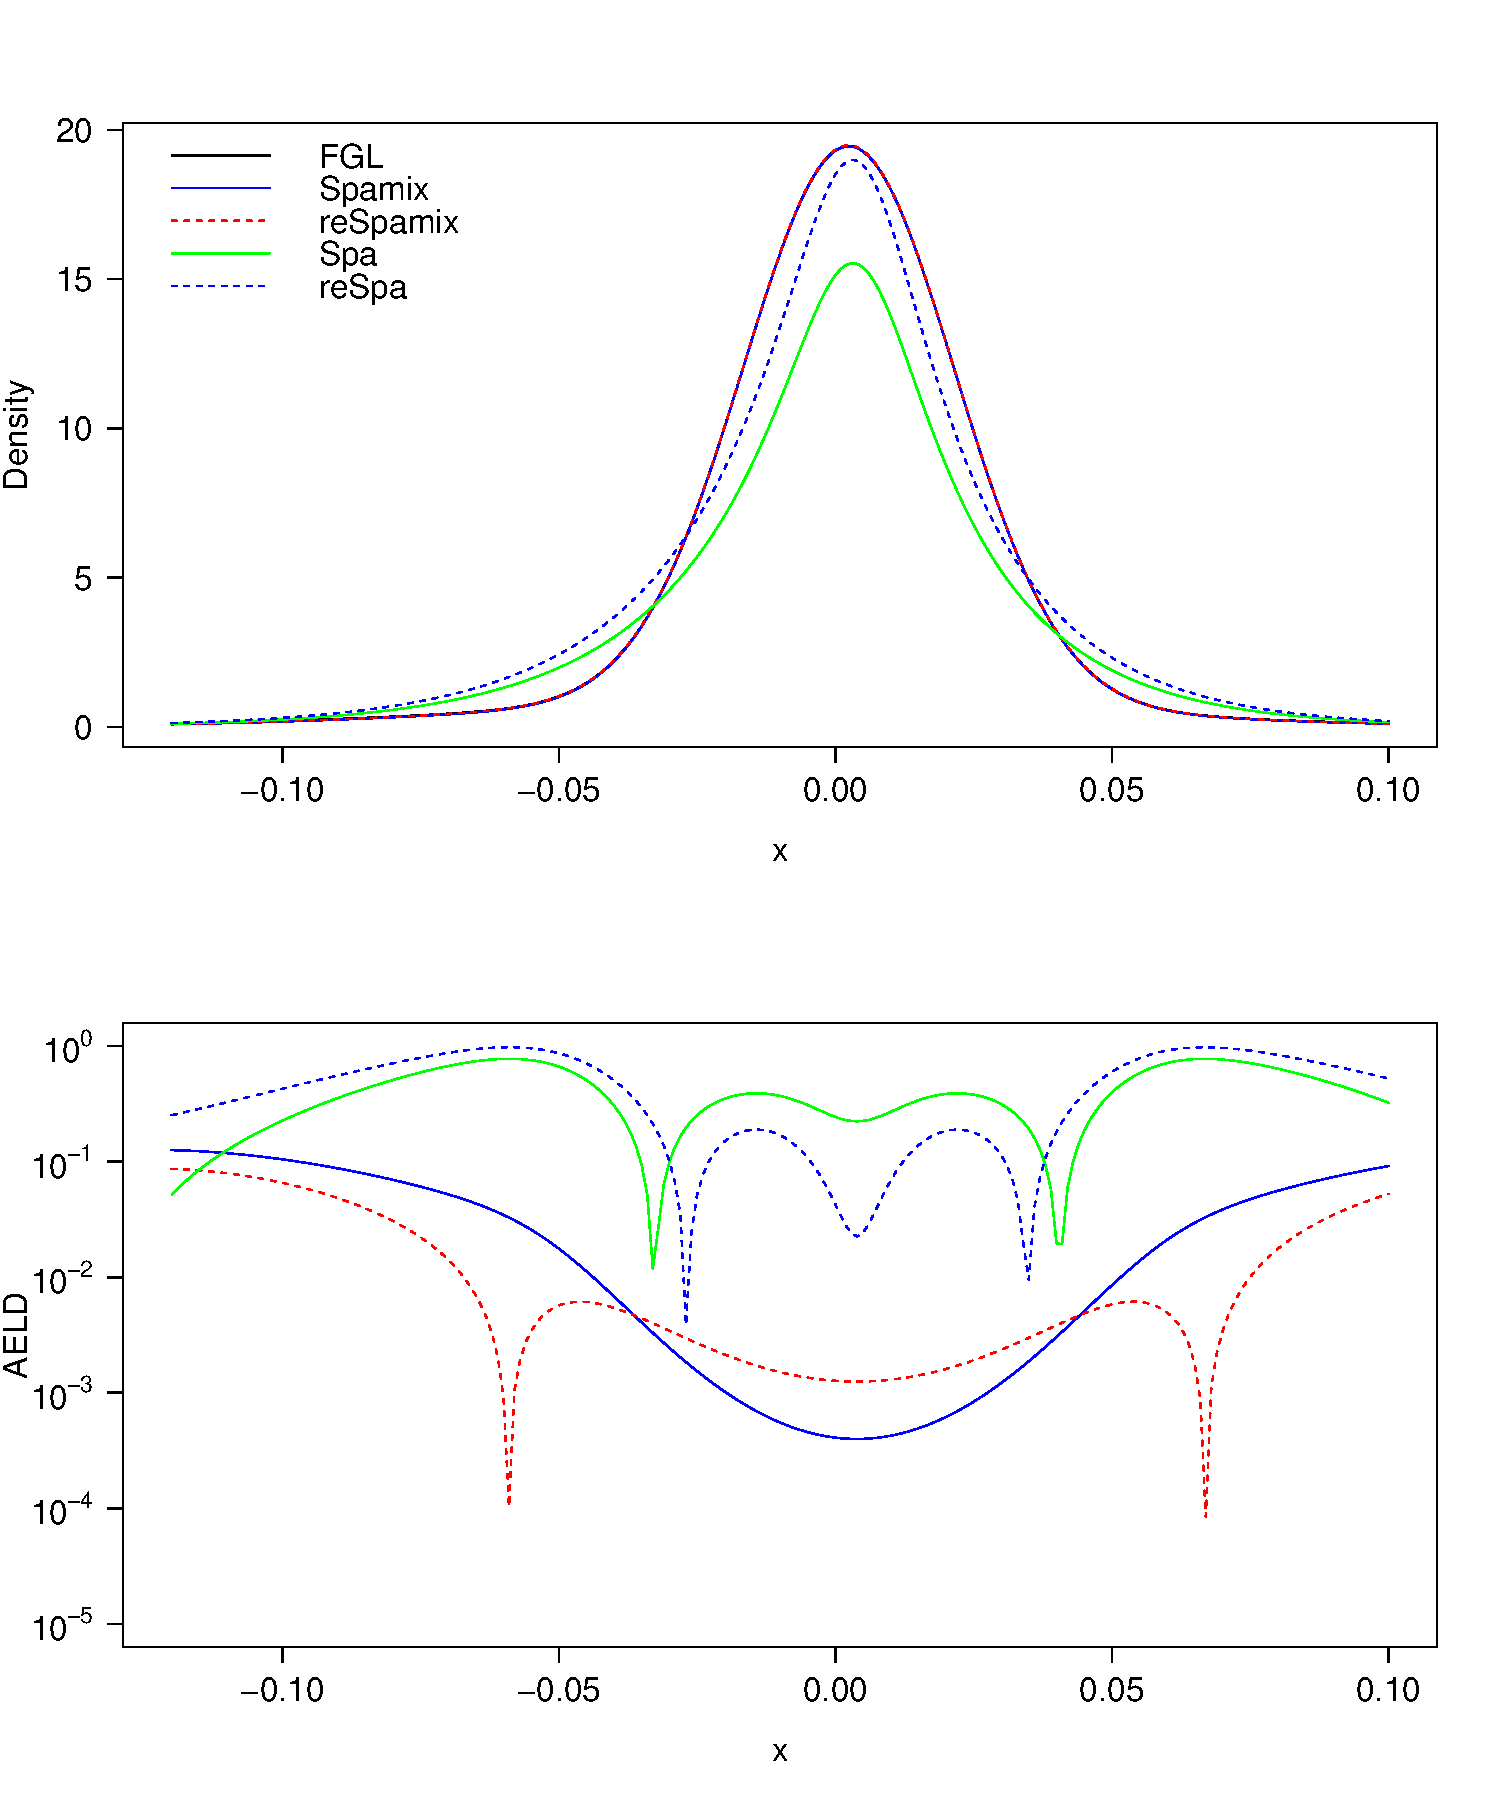
\includegraphics[width=13cm,height=12cm]{./Figures/tdmjdreal.pdf}
	\rule{35em}{0.5pt}
	\caption[Transition densities: Merton jump-diffusion]{(Top) Exact and estimated transition densities for the MJD model (for log-returns) with timestep $t=1/250$ and parameters $r=0.55$, $\sigma=0.2$, $\lambda = 18$, $\mu=-0.01$, and $\nu=0.04$.\\
		(Bottom) AELD plotted for the same values of the estimated transition densities.}\label{fig: tdmjd1}
	\label{fig: tdmjd1}
\end{figure}

\begin{figure}[htbp]
	\centering
	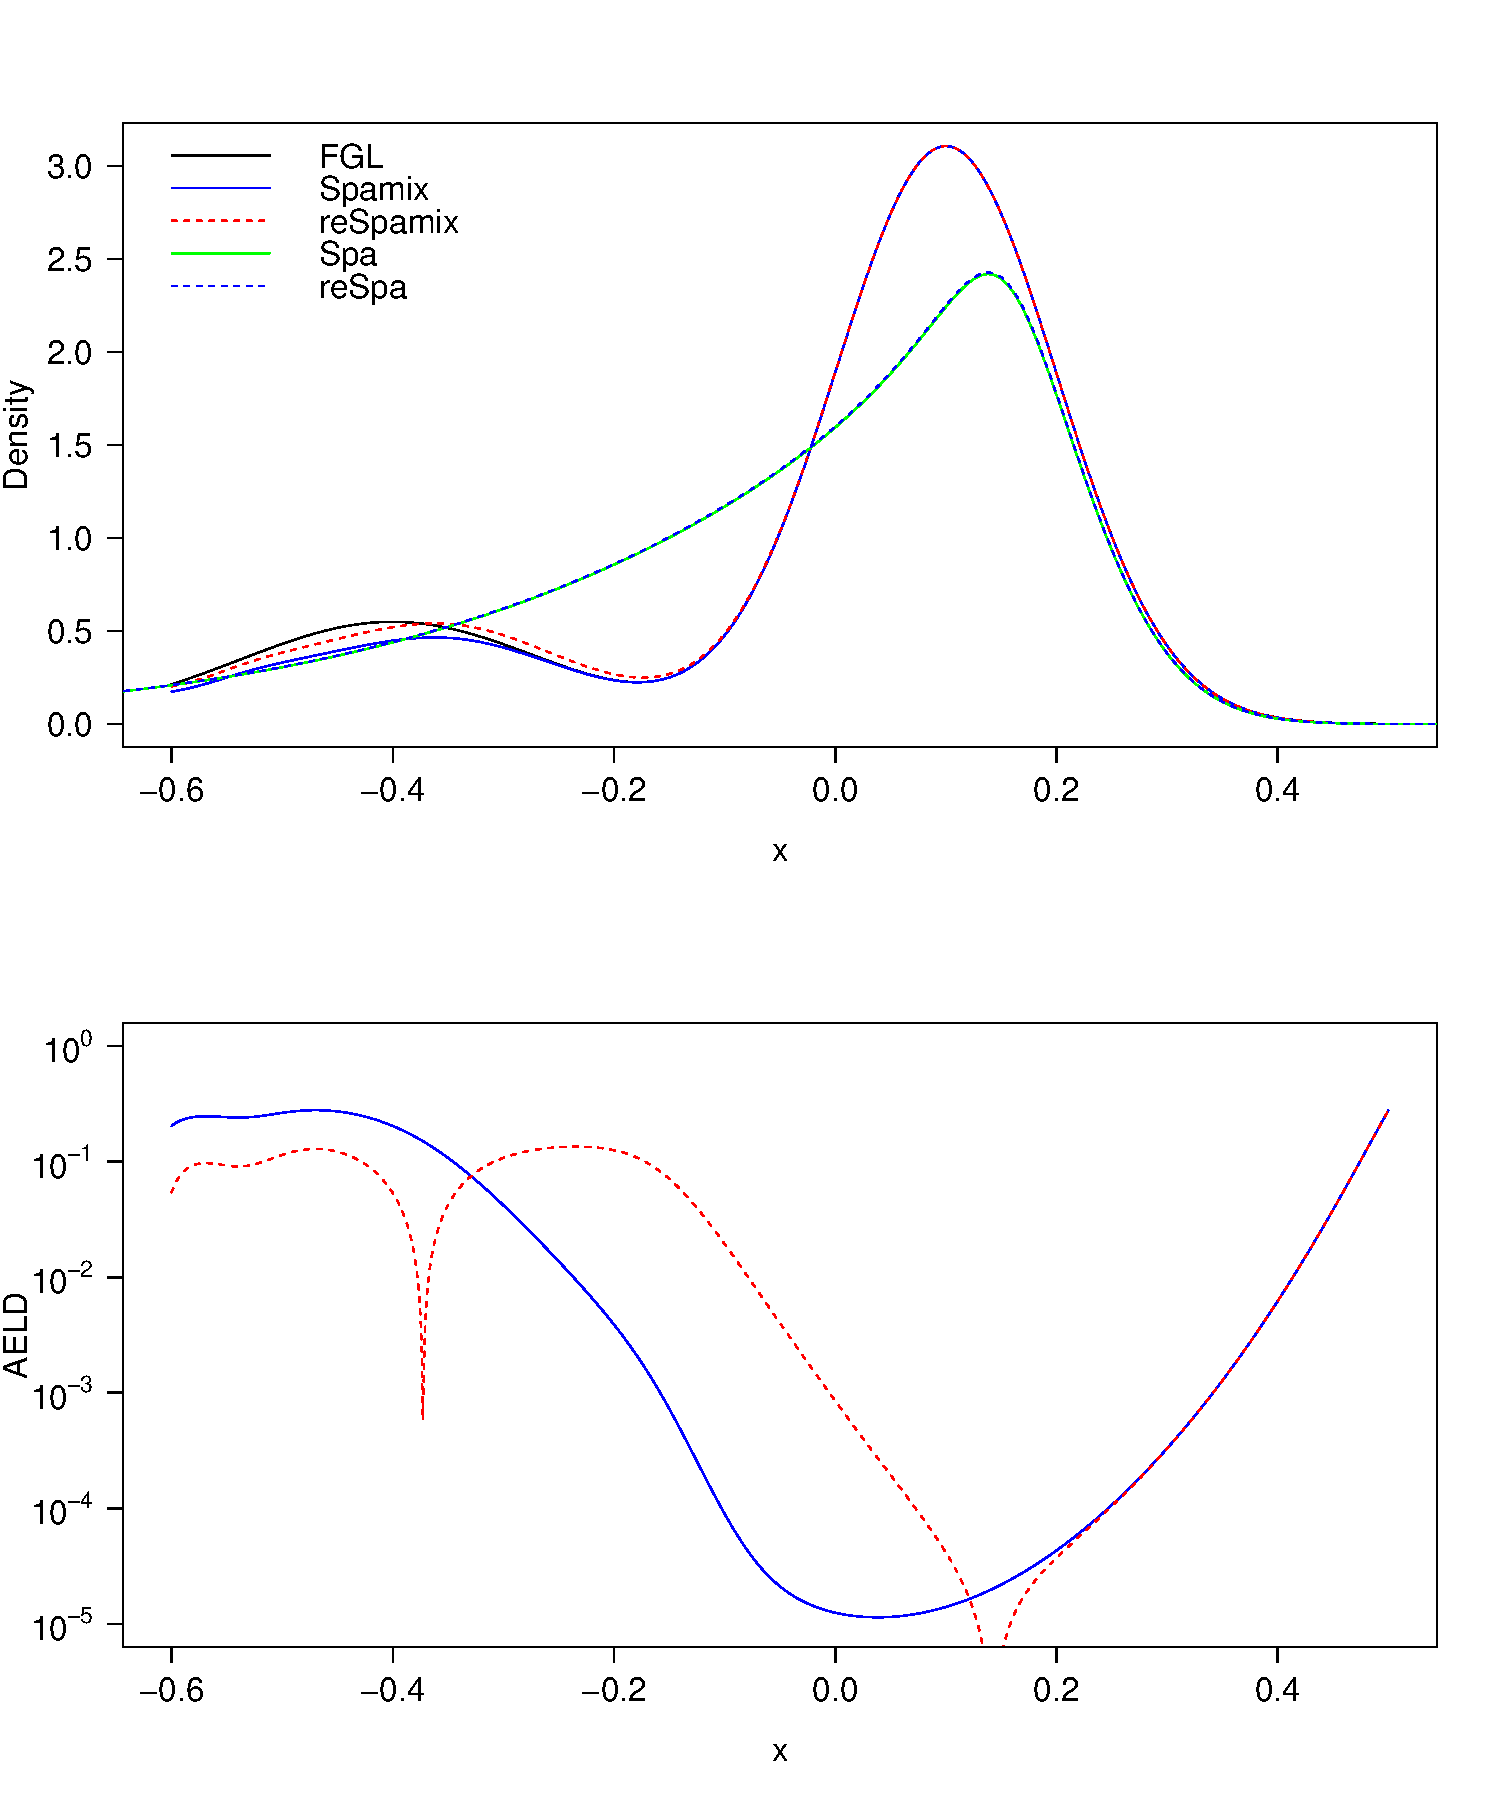
\includegraphics[width=13cm,height=10cm]{./Figures/tdmjdbimodal.pdf}
	\rule{35em}{0.5pt}
	\caption[Transition densities: bimodal Merton jump-diffusion]{Example of bimodal transition density for the MJD model (for log-returns) with timestep $t=1/4$ and parameters $r=0.03$, $\sigma=0.2$, $\lambda = 1$, $\mu=-0.5$, and $\nu=0.1$.}\label{fig: tdmjdbimodal}
\end{figure}

In the following, we present some numerical results from estimating transition densities with the ITSPA \eqref{theorem: itspa}, the mITSPA \eqref{theorem: mitspa}, and the FGL \eqref{theorem: FGL} methods.
We consider the CIR process \eqref{Chap2.3.3 (CIR)}, also considered in \citet{preston2012approximation}, and the MJD model \eqref{Chap2.3.4 (MJD)} for log-returns as our test processes for a pure diffusion and a jump-diffusion process respectively.
For the CIR process, we already have the exact transition density, for the MJD model we obtain the transition density via the FGL method, which we take as our benchmark because the characteristic function is known in closed form.
The error is measured using the absolute error of the log density (AELD), defined as
\begin{align}
\text{AELD}(x_t|x_0,\theta)&=\left|\log\hat{f}_X{t}(x_t|x_0,\theta)-f_X{t}(x_t|x_0,\theta)\right|.
\end{align}
From figure %\ref{fig:transDensAELDCIR1} 
\ref{fig: tdcir1}
we see that all approximations are close to the exact transition density.
For this particular example, it is evident that scheme 3 \eqref{Chap4 Sec1.3 Order 1.5 scheme} outperforms the Euler-Maruyama scheme \eqref{Chap4 Sec1.1 euler scheme} and the Milstein scheme \eqref{Chap4 Sec1.2 Milstein scheme}.
In view of the AELD, the renormalized version of scheme 3 seems to provide the best approximation for most points.
There are, however, points where the Milstein scheme and even the Euler-Maruyama scheme outperform the others.
This stems from the fact that at some point $\hat{f}-f$ will change sign and make the error practically zero.
For both figure \ref{fig: tdcir1} and figure \ref{fig: tdcir2}, the FGL is practically the same as the renormalized SPA.
This suggests that the error stems from the Itô-Taylor approximation, and not from the saddlepoint approximation, when considering processes without jumps.
This seems to hold for both the Milstein scheme and scheme 3.

For a different (and perhaps rather artificial) set of parameters, we see that the AELD in figure %\ref{fig:transDensAELDCIR2} 
\ref{fig: tdcir2}
is much larger than for the previous example.
The shape of the estimated transition densities for both scheme 1 and scheme 2 seems to deviate from the exact density.
The shape provided by the estimation via scheme 3 seems to be more in accordance with the exact density.
For the left tail, the AELD measurements are very similar, while for the right tail scheme 3 provides a better estimate.
Scheme 3 outperforms the others clearly where the density has the most mass.
Thus, in general, scheme 3 provides the better estimate, but there exist points (close to where $\hat{f}-f$ changes sign) where scheme 1 and scheme 2 perform better.

In figure %\ref{fig:transDensAELDmjd} 
\ref{fig: tdmjd1}
we see the exact and estimated transition densities for the MJD model for log-returns.
For this particular example, the drift and diffusion coefficients are constants, and all schemes will therefore provide exact estimates for this instance.
As noted earlier in this section, we here take the FGL approximation as our benchmark.
%Due to the large difference from the ITSPA estimate and the renormalized version, it is clear that a renormalization is necessary for likelihood-based inference for jump-diffusions.
It is evident from both the transition density plot and the AELD that the ITSPA and also its renormalized version perform poorly compared to the other methods.
The ITSPA and the renormalized version seem to have fatter tails and sharper peaks compared with the others.
The peak of the renormalized version is also very close to the peak of the exact density, as can be seen from the AELD changing sign at this point.
The reason why the mITSPA is preferable to the ITSPA is evident from both the plot of the transition density and the AELD.
The renormalized version of the mITSPA is the following approximation:
\begin{align}
\text{remspa}\left(f_{\widetilde{X}_t};x\right) = \text{spa}\left(f_{\widetilde{X}_{t^-}};x\right)e^{-\lambda t} + 
\frac{	\text{spa}\left(f_{\widetilde{X}_t^*};x\right)}{\int 	\text{spa}\left(f_{\widetilde{X}_t^*};x\right) dx}
\left(1-e^{-\lambda t}\right),
\end{align}
so the SPA for $\widetilde{X}_{t}^*$ is renormalized, but not the pure diffusion part.
The reason why we do not renormalize the whole expression is evident from figure \ref{fig: tdmjdbimodal}.
%A pitfall for the ITSPA is illustrated in figure %\ref{fig:transDensMJDBiMod}.
For some parameters, the MJD model will be bimodal, which is a shape the ITSPA is not able to replicate.
Both the mITSPA and its renormalized version perform very well for the right part (to the right of -0.1),
but the mITSPA underestimates the impact of jumps.
The renormalized version handles this problem well.
With these results in mind, we continue with the mITSPA and the DFT as approximation methods in the next section and in chapter \ref{Chapter7}.
%It is therefore important to inspect the data to check whether a bimodal distribution is reasonable, before doing likelihood-based inference on a given dataset.




\subsection{Approximation methods applied to likelihood-based analysis}
\label{Chap6 sec: approximation methods applied to likelihood-based analysis}


\begin{table}
	\newcommand{\ra}[1]{\renewcommand{\arraystretch}{#1}}
	\ra{1.3}
	\centering
	\begin{tabular}{@{}lrrrr@{}}
		\toprule
		\multicolumn{1}{c}{Method}& & \multicolumn{2}{c}{Parameters}\\
		\cmidrule{1-1} \cmidrule{3-4}
		& & \multicolumn{1}{c}{$\mu$} & \multicolumn{1}{c}{$\sigma$} &\multicolumn{1}{c}{$l(\hat{\theta};\mathbf{x})$} \\
		\midrule
		\textbf{Exact}& Estimate & 0.04551693 & 0.20474323& 2040.185  \\
		& Standard error & 0.118292400 &0.005289691 & \\
		\textbf{ITSPA}\\
		Scheme 1& Estimate & 0.04552182  & 0.20480000  &2040.051 \\
		& Standard error & 0.118320241& 0.005291158& \\
		Scheme 2& Estimate &  0.04553684 &  0.20479341 & 2040.232\\
		& Standard error & 0.118321415& 0.005292543& \\
		Scheme 3& Estimate & 0.04551767  &  0.20475610 & 2040.232 \\
		& Standard error & 0.118299834& 0.005289801&  \\
		\textbf{reITSPA}\\
		Scheme 2& Estimate &   0.04552938&  0.20478127 & 2040.235 \\
		& Standard error & 0.118314384& 0.005291601&  \\
		Scheme 3& Estimate &  0.04552016 & 0.20474397  & 2040.235 \\
		& Standard error &  0.118292829& 0.005288862&  \\
		\textbf{FGL}\\
		Scheme 2& Estimate & 0.04552548 & 0.20478043 & 2040.185 \\
		&	Standard error &0.118313815 & 0.005291554 \\
		Scheme 3& Estimate & 0.04552666 & 0.20474278 & 2040.185 \\
		&	Standard error&	0.118292071 & 0.005288793\\
		\bottomrule
	\end{tabular}
	\caption[Parameter estimates: geometric Brownian motion] {Parameter estimates for the GBM, with $\Delta t=1/250$ and $n=750$.
		True parameters are $\mu=0.1$ and $\sigma=0.2$.}
	\label{Chap6.2 GBM table}
\end{table}

\begin{table}
	\newcommand{\ra}[1]{\renewcommand{\arraystretch}{#1}}
	\ra{1.3}
	\centering
	\begin{tabular}{@{}lrrrrr@{}}
		\toprule
		\multicolumn{1}{c}{Method}& & \multicolumn{3}{c}{Parameters}\\
		\cmidrule{1-1} \cmidrule{3-5}
		& & \multicolumn{1}{c}{$\kappa$} & \multicolumn{1}{c}{$\alpha$} & \multicolumn{1}{c}{$\sigma$} &\multicolumn{1}{c}{$l(\hat{\theta};\mathbf{x})$} \\
		\midrule
		\textbf{Exact}& Estimate & 0.6371062 & 0.4767801& 0.2056826 & 1030.498 \\
		& Standard error & 0.149601549 & 0.041683387 & 0.005564301\\
		\textbf{ITSPA}\\
		Scheme 1& Estimate & 0.6204889  &  0.476780  &  0.2003414 & 1030.498 \\
		& Standard error & 0.141866267& 0.041683387& 0.005279164& \\
		Scheme 2& Estimate &  0.6204889 &  0.4767801 & 0.2003414& 1030.498\\
		& Standard error & 0.141866267& 0.041683387& 0.005279164& \\
		Scheme 3& Estimate &0.6374181  &  0.4767801&  0.2057819& 1030.498 \\
		& Standard error &0.14982442& 0.04168339&0.00557789& \\
		\textbf{FGL}\\
		Scheme 2 & Estimate& 0.6205907 & 0.4755344 & 0.1999412 & 1030.6\\
		&	Standard error & 0.141603579 & 0.041653429 & 0.005401377\\
		Scheme 3 & Estimate&0.6375256&0.4755344&0.2053718&1030.6\\
		&	Standard error &0.149548434&0.041653428&0.005697267\\
		\bottomrule
	\end{tabular}
	\caption[Parameter estimates: Ornstein-Uhlenbeck process] {Parameter estimates for the OU process with $\Delta t=1/12$ and $n=720$.
		True parameters are $\kappa=0.5$, $\alpha=0.5$, and $\sigma=0.2$.}
	\label{Chap6.2 OU table}
\end{table}



\begin{table}
	\newcommand{\ra}[1]{\renewcommand{\arraystretch}{#1}}
	\ra{1.3}
	\centering
	\begin{tabular}{@{}lrrrrr@{}}
		\toprule
		\multicolumn{1}{c}{Method}& & \multicolumn{3}{c}{Parameters}\\
		\cmidrule{1-1} \cmidrule{3-5}
		& & \multicolumn{1}{c}{$\kappa$} & \multicolumn{1}{c}{$\alpha$} & \multicolumn{1}{c}{$\sigma$} &\multicolumn{1}{c}{$l(\hat{\theta};\mathbf{x})$} \\
		\midrule
		\textbf{Exact}& Estimate & 2.6364617 & 1.0590417& 0.5287758 & 434.2396 \\
		& Standard error & 0.55194190 & 0.04644282 & 0.01766123\\
		\textbf{ITSPA}\\
		Scheme 1& Estimate & 2.5979632  & 1.0586450   & 0.5018126 & 434.2881 \\
		& Standard error &  0.49744663&0.04470062& 0.01586857& \\
		Scheme 2& Estimate &  2.4631499 & 1.0590665 & 0.5033727& 434.2972\\
		& Standard error & 0.49845482& 0.04734476& 0.01598954& \\
		Scheme 3& Estimate & 2.6323468  &1.0591018 &0.5305189&434.7113 \\
		& Standard error & 0.55584460& 0.04667515& 0.01792541& \\
		\textbf{reITSPA}\\
		Scheme 2& Estimate &  2.4630148& 1.0589346 &0.5029161& 433.8832 \\
		& Standard error & 0.49801072&0.04729622&0.01594586& \\
		Scheme 3& Estimate & 2.6198579 & 1.0593195  &0.5297991& 434.2021 \\
		& Standard error & 0.55459115& 0.04684416&0.01784453& \\
		\textbf{FGL}\\
		Scheme 2 & Estimate& 2.4625853 & 1.0845777 &0.5032077 & 433.8103\\
		&	Standard error & 0.49791928 & 0.04912341 & 0.01597505\\
		Scheme 3 & Estimate&2.6189290 &1.0592701&0.5297533&434.1375\\
		&	Standard error &0.55448542&0.04685458&0.01783991\\
		\bottomrule
	\end{tabular}
	\caption[Parameter estimates: Cox-Ingersoll-Ross process.] {Parameter estimates for the CIR process with $\Delta t=1/52$ and $n=624$.
		True parameters are $\kappa=2$, $\alpha=1$, and $\sigma=0.5$.}
	\label{Chap6.2 CIR table}
\end{table}



\begin{table}
	\newcommand{\ra}[1]{\renewcommand{\arraystretch}{#1}}
	\ra{1.3}
	\centering
	\begin{tabular}{@{}lrrrrrrr@{}}
		\toprule
		\multicolumn{1}{c}{Method}& & \multicolumn{5}{c}{Parameters}\\
		\cmidrule{1-1} \cmidrule{3-7}
		& & \multicolumn{1}{c}{$r$} & \multicolumn{1}{c}{$\sigma$} & \multicolumn{1}{c}{$\lambda$} &\multicolumn{1}{c}{$\mu$} &\multicolumn{1}{c}{$\nu$} &\multicolumn{1}{c}{$l(\hat{\theta};\mathbf{x})$} \\
		\midrule
		\\
		\multicolumn{8}{c}{\textbf{$T=1$}}\\
		\text{mitspa} &est& 0.72074&0.30700&12.86635&0.00132&0.06056&596.015\\
		&se&0.37759&0.01912&8.82091&0.02037&0.01959\\
		\text{remitspa}&est&0.72172&0.30249&16.55132&0.00040&0.05570&596.398\\
		&se&0.38265&0.02103&12.93950&0.01719&0.01938\\
		\text{FGL} &est&0.72003&0.30272&16.43486&0.00045&0.05430&596.336\\
		&se&0.37553&0.02060&12.27560&0.01644&0.01830\\
		\\
		\multicolumn{8}{c}{\textbf{$T=3$}}\\
		mitspa & est & 0.38524 & 0.30172 & 24.74671 & -0.01911 &  0.06328 & 1717.037\\
		& se& 0.25461 & 0.01067 & 5.65762 & 0.00889 & 0.00779\\
		remitspa & est & 0.36125 & 0.29691 & 29.68622 & -0.01735 & 0.05953 & 1720.067\\
		& se& 0.26023 & 0.01110 & 7.26270 & 0.00816 & 0.00734 \\
		FGL & est & 0.38405 & 0.29776 & 28.79432 & -0.01692 & 0.05882 & 1719.595\\
		& se &0.25321 & 0.01102 & 6.92008 & 0.00790 & 0.00729\\
		\\
		\multicolumn{8}{c}{\textbf{$T=5$}}\\
		mitspa & est & 0.59237 &  0.30154 & 30.57034 & 0.00051 & 0.04735 & 2897.868\\
		& se&0.17890&0.00959&6.83584&0.00484&0.00515\\
		remitspa & est & 0.59498 & 0.28530 & 52.00543 & 0.00060 & 0.03925 & 2904.966\\
		& se &0.18215&0.01220&15.40468&0.00339&0.00509\\
		FGL & est &0.59175 & 0.28959 & 45.15461 & 0.00054 & 0.04058 & 2903.782\\
		& se &0.17819 & 0.01099 & 11.49991 & 0.00360 & 0.00457\\
		\bottomrule
	\end{tabular}
	\caption[Parameter estimates with standard deviations: Merton jump-diffusion model for log-returns] {Parameter estimates (est) with standard deviations (se) for the MJD model for log-returns with $T=1$, $T=3$, and $T=5$, and $\Delta t=1/250$.
		True parameters are $r=0.4$, $\sigma=0.3$, $\lambda=30$, $\mu=-0.01$, and $\nu=0.05$.}
	\label{tab: mjdsim}
\end{table}


\begin{table}
	\newcommand{\ra}[1]{\renewcommand{\arraystretch}{#1}}
	\ra{1.3}
	\centering
	{\setlength{\tabcolsep}{0.20em}
		\begin{tabular}{@{}lrrrrrrrrr@{}}
			\toprule\\
			\multicolumn{1}{c}{Method} & \multicolumn{3}{c}{$l_\theta$} & \multicolumn{3}{c}{$\nabla_\theta l$} & \multicolumn{3}{c}{$\mathbb{H}_\theta$}\\
			\cmidrule(r){1-1}	\cmidrule(r){2-4} 	\cmidrule(r){5-7} 	\cmidrule(r){8-10}\\
			& $Q_1$ & $Q_2$ & $Q_3$ & $Q_1$ & $Q_2$ & $Q_3$ & $Q_1$ & $Q_2$ & $Q_3$  \\
			\midrule\\
			
			\multicolumn{10}{c}{\textbf{CIR}}\\
			
			\textbf{ITSPA}\\
			scheme 1 & 1.874 & 1.888 & 1.952 & 7.063  & 7.196 & 7.496 & 51.071  & 51.400 & 52.249 \\
			scheme 2 & 3.169 &3.182 &3.220 &     11.270&11.483 &11.606 &   72.521 &73.114 &73.738  \\
			scheme 3 &   4.559  &4.689 &4.841 &       15.091 & 15.445 &15.799 &  94.724 & 95.580 &97.269  \\
			
			\textbf{reITSPA}           \\
			scheme 2 &   134.809 &137.473 &141.612 &  457.098  &509.000 &584.649 &  6292.039 & 6298.884 &6301.882      \\
			scheme 3 &  173.784 &174.192 &175.156 &  591.581 &607.021 &619.613 &  4275.437 &  4563.417 & 5471.84      \\
			
			\textbf{FGL}\\
			scheme 2 & 7.417 & 7.489 &7.536 &   16.14098 &16.445 &16.777 & 78.665 &78.742 &79.279          \\
			scheme 3 &  24.527&24.666 &25.682 &   56.484 &57.116 &58.173 &  273.357&273.790 &274.896        \\
			
			\multicolumn{10}{c}{\textbf{MJD}}\\
			
			\textbf{mSPA} & 9.376 &9.488 & 9.711 & 35.335 & 35.574 & 35.986 & 389.262 &396.939 &410.138  \\
			
			\textbf{remSPA} & 150.614 &151.196 &152.677 &   539.840 &541.689 &543.621 &  8255.338 &12120.45 &12138  \\
			
			\textbf{FGL} &  15.985 &16.336 &16.666 & 35.778 & 36.031 &36.344 & 217.680 &219.360 &220.330         \\
			
			\bottomrule
		\end{tabular}}
		\caption[Microbenchmarking approximation methods] {Microbenchmarking approximation methods for the CIR process and the MJD model for log returns.
			The time (in milliseconds) it takes to evaluate the log likelihood, the gradient, and the Hessian matrix for the approximation methods.
			Evaluation of each expression was replicated 100 times, and the quartiles for each method and expression are shown in the table.
			The data used were simulated exactly, for the CIR process: 500 equidistant data points with $T=20$,
			for the MJD model: 750 equidistant data points with $T=3$.
			Parameters for both processes were set to the same values as the ones used for testing accuracy in tables \ref{Chap6.2 CIR table} and \ref{tab: mjdsim}.
			The ITSPA used 3 Newton iterations to find the saddlepoint, the renormalization used 45 points with $k=4$ (see section \ref{Chap: implementation of approx methods}).
			The mITSPA used 4 Newton iterations to find the saddlepoint, the renormalization used 25 points with $k=2.8$.
			The FGL for the CIR process was used with $n=60$, and for the MJD model: $n=70$.
		}
		\label{tab: microbenchmark}
	\end{table}
	
	
	
	In the following we present likelihood-based estimation of parameters using the methods previously discussed.
	This is compared to estimation based on using the exact transition densities, or the FGL in the case of the Merton model.
	The estimation results for the GBM, the OU process, the CIR process, and the Merton model are found in tables 
	\ref{Chap6.2 GBM table}, \ref{Chap6.2 OU table}, \ref{Chap6.2 CIR table}, and \ref{tab: mjdsim}, respectively.
	The data used for the estimation were generated using the solutions of the SDEs in chapter 
	\ref{Chap2.3}.
	The data generated were generated with timesteps $\Delta t = 1/250$ for the GBM, $\Delta t = 1/52$ for the CIR process, $\Delta t = 1/12$ for the OU process, and $\Delta=1/250$ for the Merton model, mimicking daily, weekly, and monthly observations for financial data.
	
	Considering the point estimates of the parameters and the uncertainty of these estimates, all the methods and schemes produce good results compared to the estimates based on using the exact transition densities.
	In addition, the evaluations of the log-likelihood functions in their respective optima are practically the same.
	This tells us that the renormalization of the ITSPA does not have a large and beneficial effect when one is working with pure diffusions.
	Likelihood-based inference with the ITSPA without renormalization is therefore possible and quite accurate for pure diffusions.
	This is also reasonable in view of the estimated transition densities (figures \ref{fig: tdcir1} and \ref{fig: tdcir2}) in section \ref{Chap6 sec: approximation of TD}: 
	when the timestep is small, even the Euler-Maruyama scheme \eqref{Chap4 Sec1.1 euler scheme}, which is normal, provides a reasonable approximation.
	The SPA is exact for a normal random variable, and it is therefore reasonable to assume that transition densities from higher-order schemes will be approximated accurately with the SPA, since the true (and estimated) transition densities will be close to normal.
	Renormalization does not seem to be crucial here.
	In table \ref{tab: mjdsim}, we estimated parameters for $T=1$, $T=3$, and $T=5$.
	As mentioned, renormalization of the mITSPA seems to be necessary both for parameter estimates and especially the value of the likelihood.
	
	In table \ref{tab: microbenchmark} we compare the speed (in milliseconds) of the different methods relative to each other.
	The methods involving saddlepoint approximations without renormalization (ITSPA and mITSPA) are faster than saddlepoint approximations with renormalization and also faster than the FGL method, which is second in speed. These results are valid for both the CIR process and the MJD model.
	It is also interesting to note how much more time the calculation of the gradient and the Hessian matrix is consuming than the log-likelihood function.
	Having compared both speed and accuracy, it seems natural to suggest the ITSPA method over the others when working with pure diffusion processes. In addition to being efficient and accurate, it seems to be even more stable than the FGL method, when working with the real data and diffusion models in chapter \ref{Chapter7}.
	However, for jump-diffusion processes, the FGL method is preferable compared to the other methods. It is not as fast as the mITSPA, but it provides better accuracy. Compared to the renormalized mITSPA, it is faster, more accurate and also allows for higher jump intensities without crashing.



\section{Case studies}
\label{sec::case_studies}
In this section we analyse financial data, using the approximation methods presented in chapter \ref{Chapter4}.
The first section concerns a brief presentation of some background theory and stylized facts for financial data, such as non-constant volatility and heavy-tailed return series.
%Some of these traits have been incorporated 
The standard GBM model has been extended with certain features, such as jumps (the MJD model \ref{Chap2.3.4 (MJD)}) and stochastic volatility (the Heston or Bates models), to incorporate some of these traits of financial data.
But to our knowledge nonlinearity in the price process has not been thoroughly investigated.
An exception from this is the \textit{constant elasticity of variance} model (CEV) \cite{cox1975notes}, which allows for nonlinearity in the diffusion component of the SDE.
The aim of this chapter is to investigate whether such nonlinearity is appropriate or not.
The first section considers background theory.
The likelihood-based analysis for stock prices modelled with nonlinear SDEs with and without jumps is carried out in section 2.
In section 3 we briefly compare some models for stochastic volatility. 



%A nice feauture of the approximation methods presented in chapter \ref{Chapter4}, as shown in chapter \ref{Chapter6}, is its possibility of likelihood-based inference for any diffusion process driven by a SDE, on the conditioned that the timestep is not too large.

%The standard GBM model has been extended with features, such as jumps (the MJD model) and stochastic volatility to incorporate some of these traits of financial data.
%However, to our knowledge, nonlinearity in the price process has not been investigated.
%The goal of this chapter is therefore to extend the GBM and the MJD models to a broader class of nonlinear models, and then perform likelihood-based analysis using the ITSPA, in order to be able to conclude whether our new class of models fit the data significantly better than the former.




\subsection{Background Theory}

Most financial models have their basis in the \textit{efficient market hypothesis} (EMH).
This hypothesis states that markets are informatively efficient, in the sense that all available information is incorporated into asset prices.
Therefore it is in this context impossible to consistently achieve returns in excess of average market returns on a risk-adjusted basis \citep[Chapter 13, p.~317]{brealey2012principles}.
EMH depends upon several assumptions made about the market and its participants. 
One of the most important (and frequently discussed) of those is the rationality assumption made about agents in the markets.
It can be formalized in terms of Bayesian statistics:
\begin{enumerate}
	\item Agents hold a prior probability belief over states of the world.
	\item Agents obtain new information about individual stocks or about macroeconomic events.
	\item Agents update their prior probability belief to form a posterior probability belief using Bayes' law.
\end{enumerate}
Stock price models such as the GBM \eqref{Chap2.3.1 (GBM)} and the Merton model \eqref{Chap2.3.4 (MJD)} are compatible with EMH.

To discuss the appropriateness of EMH, some \textit{stylized facts} for financial data are needed, based upon inferences drawn from empirical observations concerning log-returns for equities, indices, exchange rates, and commodity prices \citep{mcneilquantitative}:
\begin{enumerate}\label{Chap7 stylized}
	\item Return series are not iid, although they show little serial correlation.
	\item Series of absolute or squared returns show profound serial correlation.
	\item Conditional expected returns are close to zero.
	\item Volatility appears to vary over time.
	\item Return series are heavy-tailed.
	\item Extreme returns appear in clusters. 
\end{enumerate}
In the framework of the EMH, large price jumps and rare events are often incorporated using the "Black Swan" concept developed by Nassim Taleb \citep{taleb2010black}.
This can be incorporated in the GBM model by extending the SDE with a jump component, leading to e.g. the Merton model if jumps are lognormally distributed.
Stochastic volatility has been incorporated via choosing the instantaneous variance in the GBM model to follow a CIR process \eqref{Chap2.3.3 (CIR)}, this is known as the Heston model \citep{heston1993closed}.
The combination of the Heston model and the Merton model is known as the Bates stochastic volatility jump-diffusion model \citep{bates1996jumps}.
However, some of the other facts are difficult to deal with in the framework of EMH.
If log-returns are not iid, then the random walk hypothesis breaks down, and if log-returns are iid and heavy-tailed, the GBM model is not a suitable model.
We do however note that for longer time intervals such as months and years, return series seem to behave more as iid random variables \citep{mcneilquantitative}.

A somewhat different approach to financial modelling is proposed in \citet{johansen2000crashes, sornette2002nonlinear, lin2009consistent}.
They view financial markets as complex systems where investors interact with each other.
The perhaps most interesting part is the notion of nonlinear behaviour of stock prices due to positive reinforcement or herding behaviour (violating the rationality assumption) leading to crashes as critical points.
According to \citet{johansen2000crashes}, the easiest way to describe a mimicking process, $S_t$, is in accordance with the equation 
\begin{align}
dS_t=rS^\alpha,
\end{align}
where $\alpha>1$ \citep{johansen2000crashes}.
It is then possible to use this description to extend standard stock price models.
The "natural" extension of the geometric Brownian motion,
\begin{align}\label{Chap7.1 eGBM}
dS_t = rS_t^\alpha dt + \sigma S_t^\alpha dW_t,
\end{align}
is proposed in \citet{sornette2002nonlinear}, but is there not further investigated.
Instead they propose a similar model containing parts ”as a convenient device to simplify the Itô calculation of these stochastic differential equations” \citep{sornette2002nonlinear}.
Such additions with no economic interpretation might be considered unaesthetic and makes the model less attractive.
But with the methods discussed in chapter \ref{Chapter4}, we can extend and analyse the standard stock-price models to nonlinear models in a natural way.
%However, with the ITSPA \ref{th it is possible to extend the GBM model in the natural way.
A model similar to \eqref{Chap7.1 eGBM} is the CEV model, where only the diffusion part is allowed to be nonlinear.
Table \ref{tab: stock price models} gives an overview over the models to be investigated.


\begin{table}
	\newcommand{\ra}[1]{\renewcommand{\arraystretch}{#1}}
	\ra{1.3}
	\centering
	{\setlength{\tabcolsep}{0.35em}
		\begin{tabular}{@{}lrrr@{}}
			\toprule
			\multicolumn{1}{c}{Model name} & 
			\multicolumn{1}{c}{Drift component} & 
			\multicolumn{1}{c}{Diffusion component} & 
			\multicolumn{1}{c}{Jump component} \\
			\cmidrule(r){1-1} \cmidrule(r){2-2} \cmidrule(r){3-3} \cmidrule(r){4-4} \\
			GBM & $rS_t$ & $\sigma S_t$ & None \\
			CEV & $rS_t$ & $\sigma S_t^\alpha$ & None \\
			nlModel 1 & $rS_t^\alpha$ & $\sigma S_t^\alpha$ & None \\
			nlModel 2 & $rS_t^\alpha$ & $\sigma S_t^\beta$ & None \\
			MJD & $(r-\lambda\hat{k})S_t$ & $\sigma S_t$ & Log-normal \\
			CEVJD & $(r-\lambda\hat{k})S_t$ & $\sigma S_t^\alpha$ & Log-normal \\
			\bottomrule
		\end{tabular}
	}
	\caption[Stock price models]{Stock price models considered in the preceding section.
		The first nonlinear model (nlModel 1) is the model described by equation \eqref{Chap7.1 eGBM}, the second nonlinear model (nlModel 2) is a refinement where the exponent is allowed to be different for the drift and diffusion coefficients. The constant elasticity of volatility jump-diffusion (CEVJD) model is the CEV model extended with a log-normal jump component.} \label{tab: stock price models}
\end{table}







\subsection{Analysis of Stock Prices as Nonlinear Processes}

\begin{table}
	\newcommand{\ra}[1]{\renewcommand{\arraystretch}{#1}}
	\ra{0.9}
	\centering
	{\setlength{\tabcolsep}{0.20em}
		\begin{tabular}{@{}lrrrrrrrrrrr@{}}
			\toprule
			\multicolumn{1}{c}{Model}& & \multicolumn{6}{c}{Parameters} & \multicolumn{3}{c}{Statistics}\\
			\cmidrule(r){1-1} \cmidrule(r){3-8} \cmidrule(r){9-11}\\
			& & \multicolumn{1}{c}{$r$} & \multicolumn{1}{c}{$\sigma$} & \multicolumn{1}{c}{$\alpha$} & \multicolumn{1}{c}{$\beta$} & \multicolumn{1}{c}{$\lambda$} & \multicolumn{1}{c}{$\mu$} & \multicolumn{1}{c}{$\nu$} &
			$l(\hat{\theta};\mathbf{x})$ & \multicolumn{1}{c}{$D$} & \multicolumn{1}{c}{p-value}\\
			\midrule
			\\
			\multicolumn{12}{c}{\textbf{SSE bubble of 07}}\\
			GBM& est & 0.6268  & 0.2629  & & & & & & 1796.7 &	&0.0013\\
			& se & 0.1604& 0.0071& & & & & & & \\
			CEV& est & 0.4718 & 0.0118 & 1.4072 & & & & & 1826.2 & 59 & 0.0011\\
			& se & 0.1478 & 0.0021 & 0.0244 \\
			nlModel 1& est & 0.0249 &  0.0112 & 1.4132 & & & & &  1827.6 & 61.8 & 0.0030\\
			& se & 0.0082& 0.0019& 0.0235& \\
			nlModel 2 & est & 0.0001 & 0.0120 & 2.0744 & 1.4046 & & & & 1828.9  & 64.4 & 0.0020\\
			& se & 0.0005 & 0.0022 & 0.3920 & 0.0247 & \\
			MJD& est & 0.6261 & 0.1694& & &  92.1& -0.0039& 0.0202& 1840.9 & 88.4 & 0.7645 \\
			& se & 0.1584& 0.0272& & & 64.9& 0.0027& 0.0051& & \\
			CEVJD & est & 0.4356 & 0.0128 & 1.3769 & & 13.6 & -0.0094 & 0.0345 & 1851.8 & 110.2 & 0.0179 \\
			& se & 0.1525 & 0.0033 & 0.0345 & &  8.2 & 0.0086 & 0.0085 \\
			\\
			\multicolumn{12}{c}{\textbf{S\&P500 Dot-com bubble}}\\
			GBM& est & 0.1817  & 0.1399  &  & & & & &  3536.6  & & 0.0021\\
			& se & 0.0460& 0.0020& & & & & & &  \\
			CEV& est & 0.1798 & 0.0095 & 1.4093 & & &  & & 3587.4 & 101.6 & 0.0087\\
			& se & 0.0420 & 0.0010 & 0.0175 & \\
			nlModel 1& est & 0.0133 &  0.0097 & 1.4072 & & & & & 3587.2 & 101.2 & 0.0098 \\
			& se & 0.0034& 0.0010& 0.0177& \\
			nlModel 2 & est & 0.1855 & 0.0095 & 0.9950 & 1.4094 & & & & 3587.4 & 101.6 & 0.0088 \\
			& se & 0.7987 & 0.0010 & 0.6829 & 0.0175 & \\
			MJD& est& 0.1797 & 0.0731& & & 118.0 & 0.0002& 0.0108 & 3580.8& 88.4 & 0.9661 \\
			& se& 0.0452& 0.0110 & & & 38.1 & 0.0005 & 0.0012 & & \\
			CEVJD & est & 0.1801 & 0.0019 & 1.6170 & &  31.1 & 0.0020 & 0.0140 & 3625.0 & 176.8 & 0.5466 \\
			& se & 0.0783 & 0.0006 & 0.0185 & & 66.3 & 0.0042 & 0.0103 &  & \\
			\\
			\multicolumn{12}{c}{\textbf{DJIA 1929 bubble}}\\
			GBM& est & 0.2328  & 0.1476  &  & & & & & 4224.8  & & 0.000009\\
			& se & 0.0647& 0.0028& & & & & & & \\
			CEV& est & 0.2205 & 0.0101 & 1.5056 & & & & & 4255.1 & 60.6 & 0.000015\\
			& se & 0.0620 & 0.0011 & 0.0227 & & \\
			nlModel 1& est & 0.0160 &  0.0101 & 1.5051 &  & & & & 4255.3& 61.0 & 0.000027 \\
			& se & 0.0048& 0.0011& 0.0228& &  \\
			nlModel 2 & est & 0.0024 & 0.0072 & 1.7331 & 1.5038 & & & & 4255.3 & 61.0 & 0.000025\\
			& se & 0.0134 & 0.0006 & 1.0447 & 0.01688 & \\
			MJD& est& 0.2223& 0.0961& & & 104.9&-0.0033& 0.0104& 4295.8& 142 & 0.9153 \\
			& se& 0.0647& 0.0057& & & 25.1 & 0.0008& 0.0008 & & \\
			CEVJD & est &  0.2234 & 0.0061 & 1.5490 & & 49.4 & -0.0047 & 0.0130 & 4315.3 & 181 & 0.3694 \\
			& se & 0.0618 & 0.0011 & 0.0394 & & 8.9003 & 0.0002 & 0.0006 & \\
			\bottomrule
		\end{tabular}}
		\caption[Parameter estimates for empirical data] {Parameter estimates (est) with standard deviations (se) for the (log) stock price models, 
			in addition to the likelihood values, 
			the $D$ statistic \eqref{eq: statistic twice log liklihood ratio} where the GBM is the model under the null hypothesis,
			and the p-values from the Kolmogorov-Smirnov test for uniformity after the transformation \eqref{eq: transform to uniformity}. }
		\label{tab: Parameter estimates stock prices}
	\end{table}
	
	\begin{figure}[htbp]
		\centering
		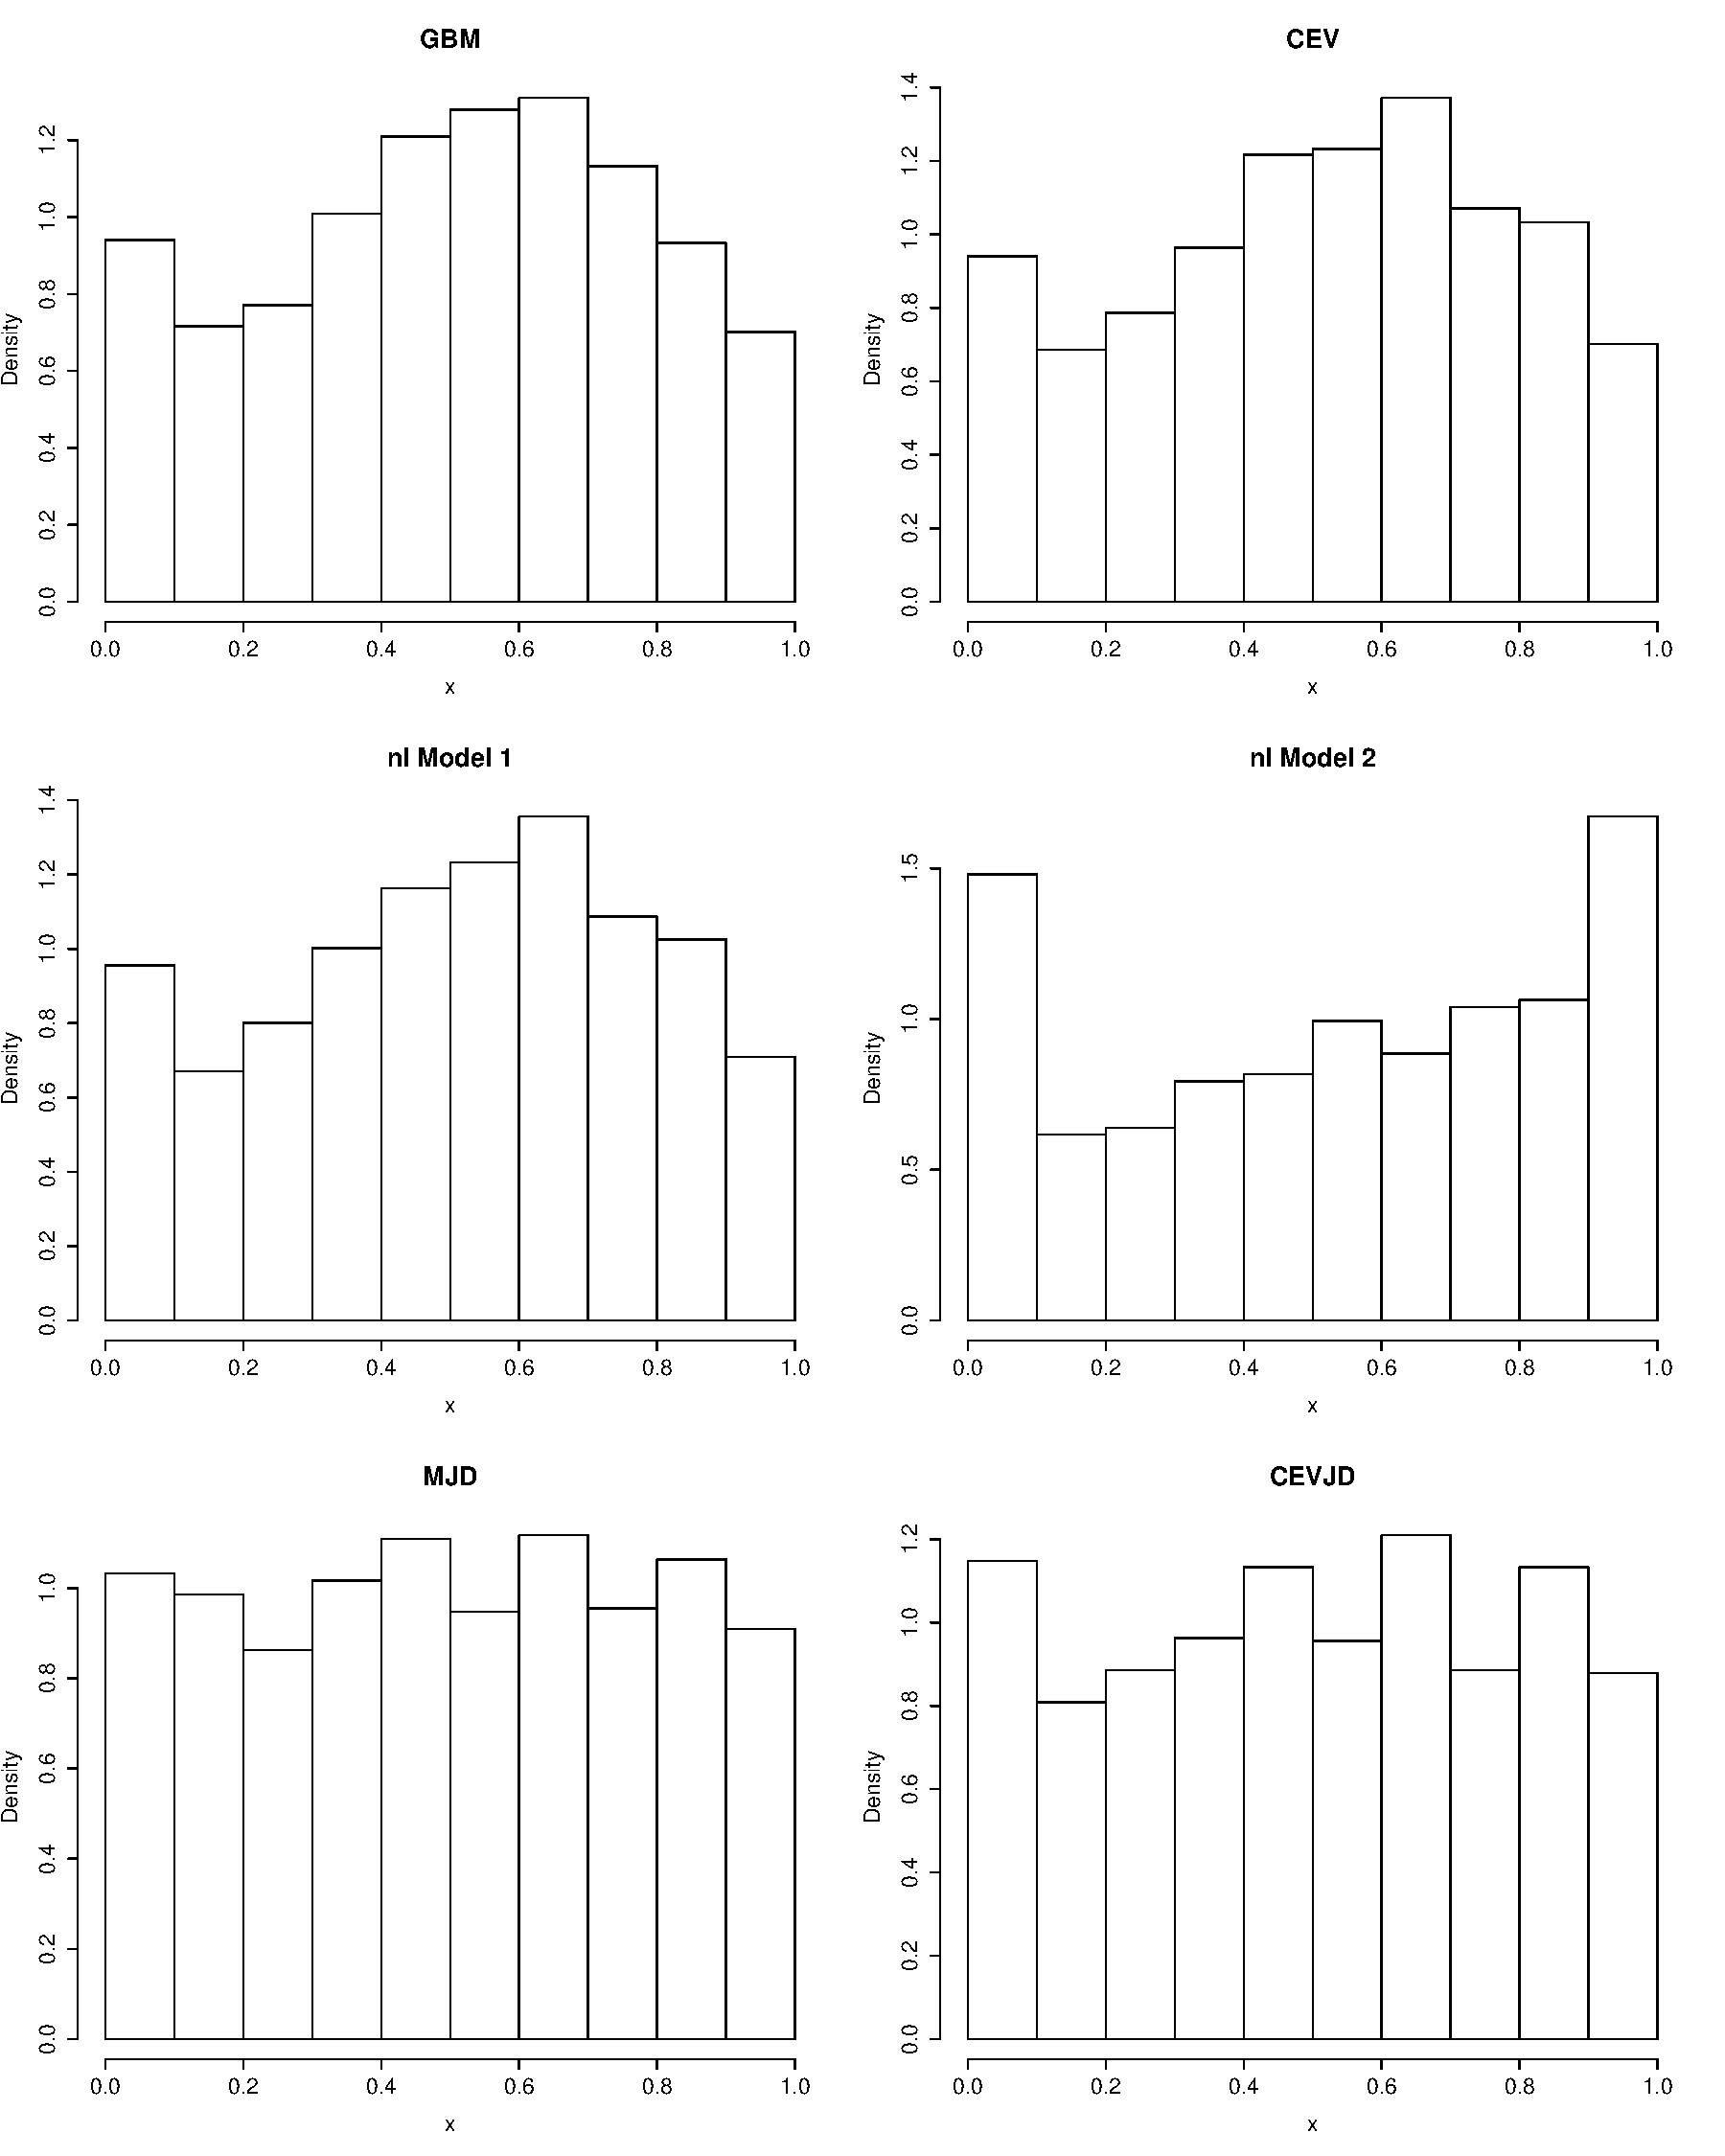
\includegraphics[width=12cm,height=13cm]{./Figures/unidiagnostic2.pdf}
		\rule{35em}{0.5pt}
		\caption[Histograms of transformed empirical data]{Goodness-of-fit diagnostic for different models. 
			Histograms of the quantity \eqref{eq: transform to uniformity} should be compared to a uniform distribution.}
		\label{fig: uniform diagnostic}
	\end{figure}
	
	\begin{figure}[htbp]
		\centering
		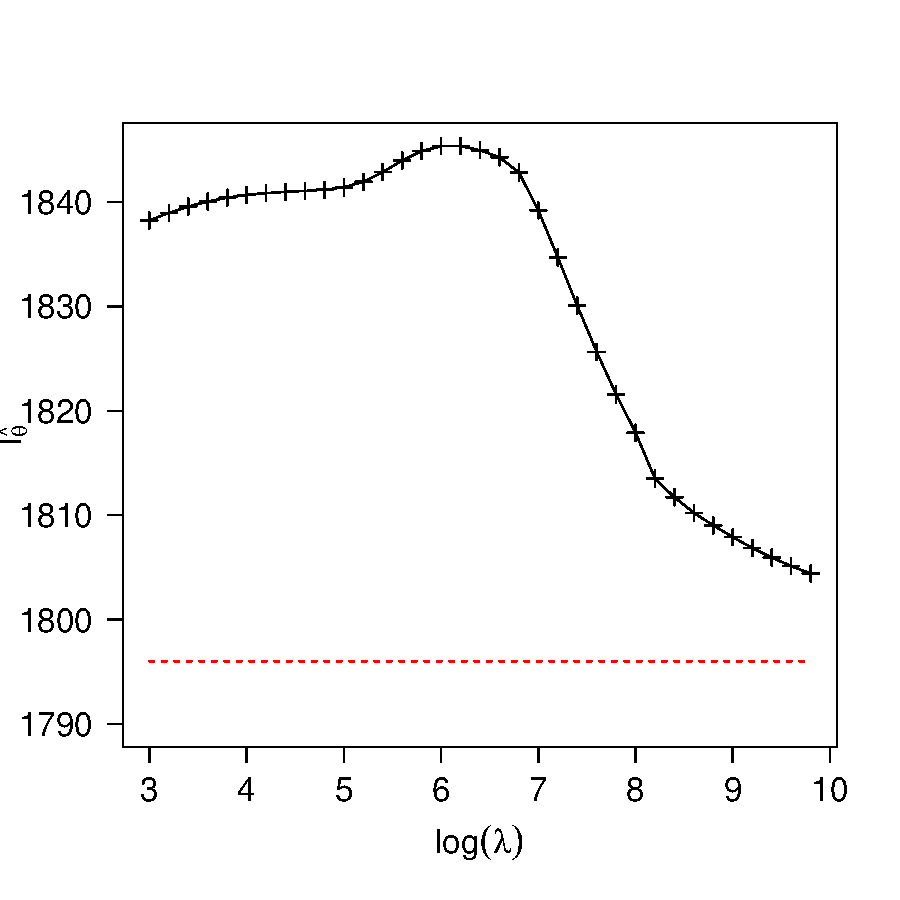
\includegraphics[width=10cm,height=8cm]{./Figures/jllvslambda.pdf}
		\rule{35em}{0.5pt}
		\caption[Profile likelihood versus logarithmic jump intensities]{Profile likelihood versus logarithmic jump intensities together with the value of the optimized GBM log-likelihood (dashed line).}
		\label{fig: jll vs lambda}
	\end{figure}
	
	
	It is interesting to investigate whether stock prices emit nonlinear behaviour ($\alpha\neq 1$).
	Using stock price data of daily returns ($\Delta t = 1/250$) on the Shanghai Securities Exchange (SSE) from 03.01.2005 until 16.10.2007, the Dow Jones Industrial Average (DJIA) from 29.04.1925 until 03.09.1929, and data from every other day ($\Delta t=1/125$) on the Standard \& Poors 500 (S\&P500) from 11.10.1990 until 24.03.2000, we estimate parameters for the models in table \ref{tab: stock price models} for different time periods and bubbles.
	In addition, we evaluate the hypothesis $H_0:\,\alpha=1$ against the alternative hypothesis $H_1:\,\alpha\neq1$ by calculating twice the log of the likelihoods' ratio (denoted by $D$), i.e.:
	\begin{align}\label{eq: statistic twice log liklihood ratio}
	D = 2\left( l(\hat{\theta}_1;\mathbf{x}) - l(\hat{\theta}_0;\mathbf{x})   \right),
	\end{align}
	where the subscripts denote the respective hypothesis,
	exploiting that the GBM and the MJD are special cases ($\alpha=1$) of their nonlinear counterparts.
	
	As a diagnostic (goodness of fit) to test whether the models are at all reasonable models for logarithmic stock prices, we transform the data in the following way:
	given a model $m$ for the logarithmic stock prices $x_1,\ldots,x_n$, the data are transformed according to
	\begin{align}\label{eq: transform to uniformity}
	y_i = F_{X_t}^m(x_i)
	\end{align}
	%$y_i=F_{X_t}^m(x_i)$ 
	for $i=2,\ldots, n$, where $F_{X_t}^m$ is the distribution function of $X_{t_i}|X_{t_{i-1}}$, given the model $m$.
	Under the assumption that the data indeed follow the model $m$, we can test the transformed data for uniformity on the interval $[0,1]$ using the Kolmogorov-Smirnov test.
	This test will however not be perfectly accurate, as it requires observations of iid random variables. Our original observations form a time series, and are not iid.
	%A possible consequence is that the p-values becomes small.
	
	All the data were transformed to logarithmic indices. 
	The models must then be transformed using Itô's lemma \ref{Chap2.2 Ito lemma jump}. 
	Using the ITSPA \eqref{theorem: itspa} with scheme 3 for the pure diffusion models, and the FGL method \eqref{theorem: FGL} also with scheme 3 for the jump-diffusions, we then estimate parameters and evaluate the log-likelihoods at the optima.
	The results can be found in table \ref{tab: Parameter estimates stock prices}, showing significant support in favour of the nonlinear models.
	Comparing the $D$ statistic with the chi-square distribution, we see that both the addition of nonlinearity and of jumps are significant improvements.
	The likelihood of the CEV model compared to the nonlinear models (nlModel 1 and nlModel 2) are very close to one another.
	From this we can not suggest that agents in the markets have so-called bounded rationality or herding behaviour as described in \cite{sornette2002nonlinear}, since the nonlinearity parameter in the drift part of the SDE is not a significant addition to the model.
	We therefore have chosen the simplest model (CEV) and have extended it with a jump component, leading to what we call the \textit{constant elasticity of variance jump-diffusion} model (CEVJD).
	This was done in order to see if the data continued to emit nonlinear behaviour, even when allowing for jumps.
	And for all three datasets this was indeed the case.
	
	The MJD model aims at modelling relatively rare events leading to abnormal changes in the stock price.
	According to this model, the jump intensity $\lambda$ should be fairly low, since by definition rare events do not happen very often.
	For all three datasets, the $\hat{\lambda}_{ml}$ estimates for the MJD model are around $100$, but for the CEVJD, the estimated jump intensities are 13.6, 31.1, and 49.4.
	A possible interpretation is the following:
	the behaviour that is captured as nonlinearity in the CEVJD model is so significant for the value of the log-likelihood of the MJD model, that instead of modelling rare events, the behaviour is captured in the jump component as several small jumps.
	The estimated jump sizes $\mu$ and variances $\nu^2$ are also greater in absolute value for the CEVJD model than for the MJD model, which supports our interpretation.
	
	The ITSPA for diffusions and the FGL method for jump-diffusions (both with scheme 3) were chosen on the basis of their speed, their stability and their accuracy.
	As mentioned in chapter \ref{Chapter6}, the SPA methods (without renormalization) are faster than the FGL methods (see table \ref{tab: microbenchmark}), and for diffusion processes without jumps they also seem to be more stable than the FGL methods (and also SPA with renormalization).
	However, when working with jump-diffusion processes, the FGL method is more accurate than the SPA method (renormalization is needed, see chapter \ref{Chapter6}), reasonably fast (faster than SPA with renormalization), and it seems to be quite stable (more stable than SPA with renormalization).
	
	As a side note, we have plotted the profile likelihood (MJD log-likelihood) %(value of the MJD log-likelihood for its optimized parameters and fixed values of lambda 
	versus the fixed values of the logarithmic lambda in figure \ref{fig: jll vs lambda}. 
	It seems that the value of the profile likelihood tends towards the value of the GBM optimized likelihood, when the jump intensity grows large. This is in accordance with theorem \ref{theorem: MJD lambda limit}.
	
	From the p-values from the Kolmogorov-Smirnov test in table \ref{tab: Parameter estimates stock prices} and the histograms in figure \ref{fig: uniform diagnostic} (bearing in mind the inaccuracy described earlier), we see that
	the data transformed with models that include the possibility of jumps are closer to a uniform distribution on $[0,1]$.
	%the inclusion of jumps are of huge importance to a good model, both the MJD and CEVJD models are not rejected on the 99\% level, but the pure diffusion models easily are.
	On the 95\% confidence level, the CEVJD model is rejected for the SSE data, while the MJD is not.
	Indeed, the p-values for transformed data under the MJD model are greater than those for the CEVJD.
	This is interesting, because the MJD is a special case of the CEVJD model, and this must imply that optimizing the value of the likelihood is not equivalent to optimizing for uniformity for the transformed data. 
	%The data transformed with models that includes the possibility of jumps can be seen to be closer to a uniform distribution on $[0,1]$.
	%Corresponding p-values from a Kolmogorov-Smirnov test can be found in table \ref{tab: Parameter estimates stock prices}.
	
	
	\subsection{Stochastic Volatility Models}
	
	\begin{figure}[htbp]
		\centering
		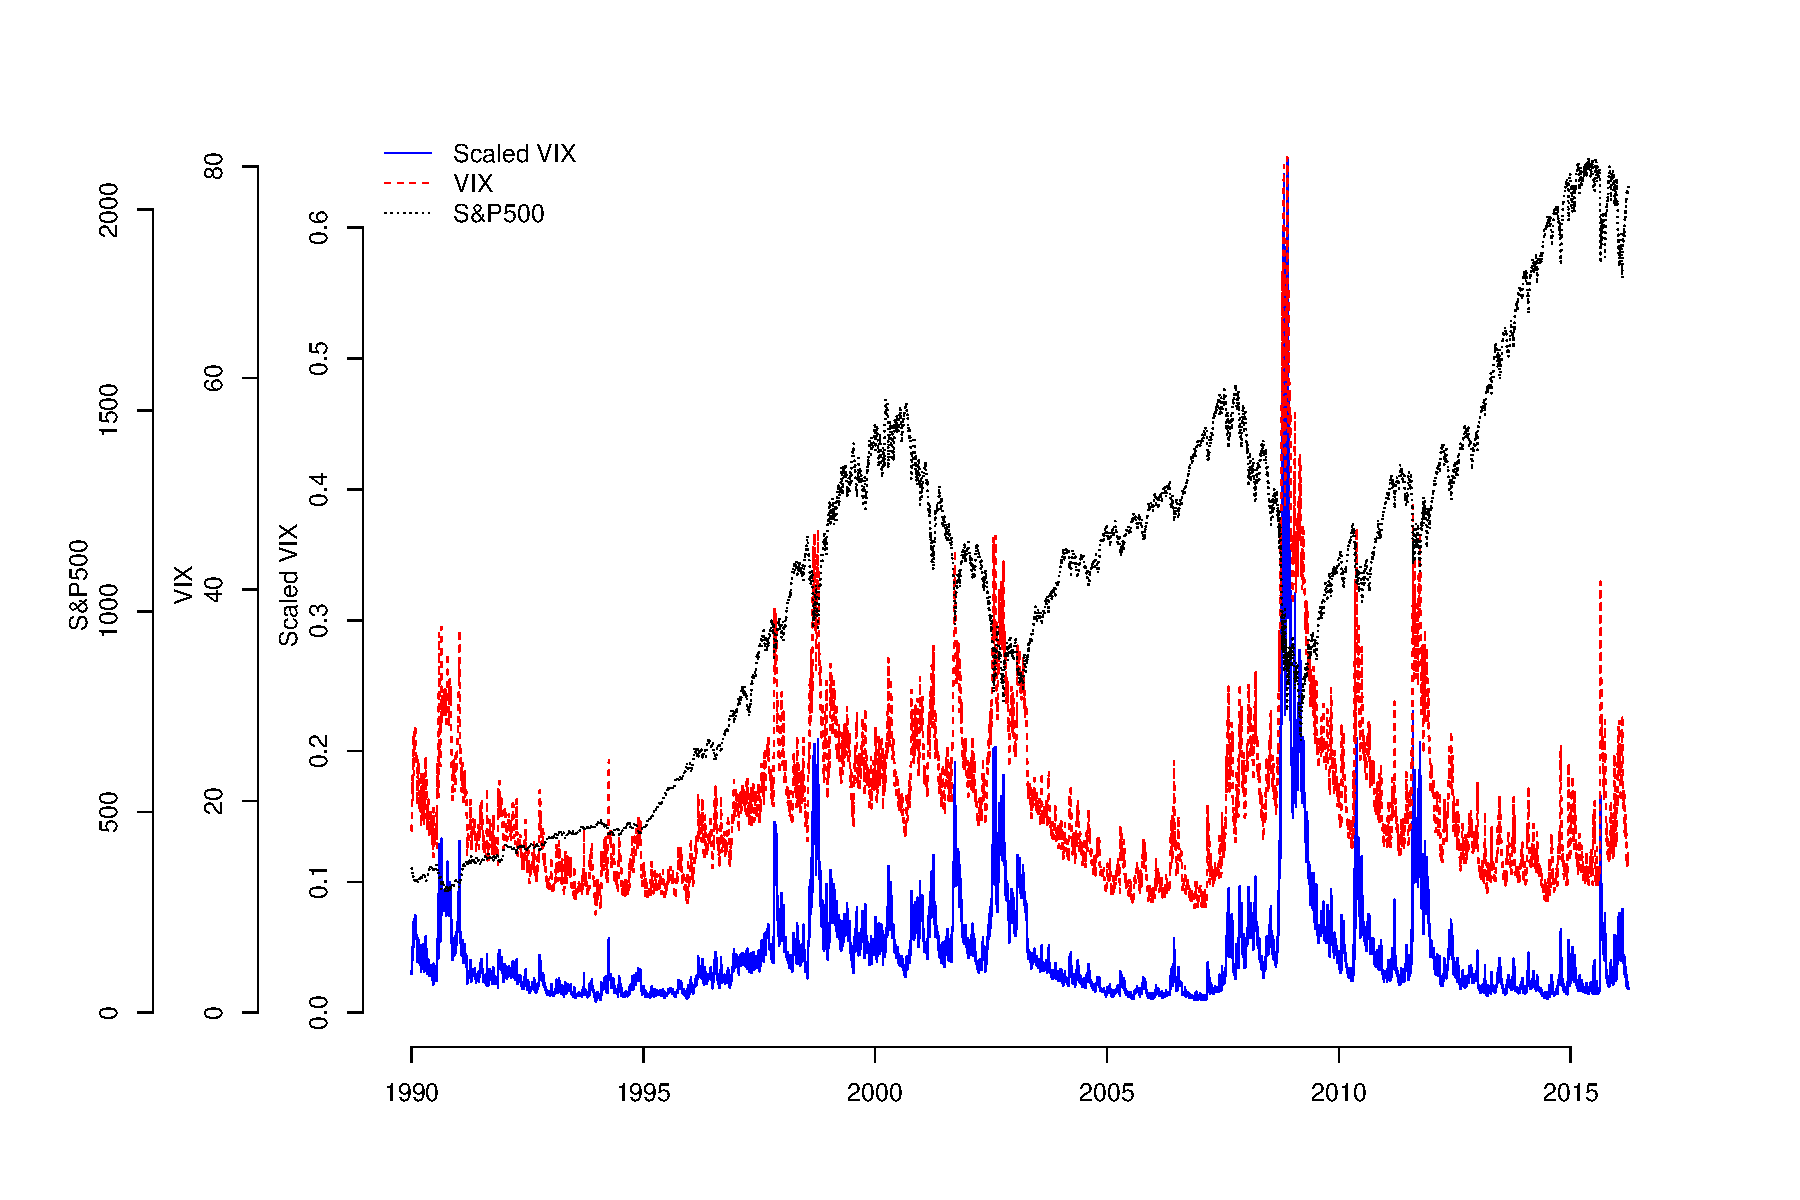
\includegraphics[width=15cm,height=8cm]{./Figures/vixSP.pdf}
		\rule{35em}{0.5pt}
		\caption[The scaled VIX for daily variance]{The scaled VIX for daily variance plotted together with the original VIX and the underlying S\&P500 indices.}
		\label{fig:vix}
	\end{figure}
	
	
	\begin{table}
		\newcommand{\ra}[1]{\renewcommand{\arraystretch}{#1}}
		\ra{1.3}
		\centering
		{\setlength{\tabcolsep}{0.35em}
			\begin{tabular}{@{}lrrrrrrrr@{}}
				\toprule
				\multicolumn{3}{c}{Model} & & \multicolumn{4}{c}{Estimates} & \multicolumn{1}{c}{Statistic}\\
				\cmidrule(){1-3} \cmidrule(r){5-8} \cmidrule(r){9-9}\\
				Name& Drift& Diffusion& & $\kappa$ & $\alpha$ & $\sigma$ & $\delta$ &  $l(\hat{\theta},\mathbf{x})$\\
				\midrule
				OU & $\kappa(\alpha - V_t)$ & $\sigma$ & est& 7.46228 & 0.04550 & 0.18001 & & 20308\\
				&	&	& se & 0.76305 & 0.00469 & 0.00158 & \\
				CIR & $\kappa(\alpha - V_t)$ & $\sigma\sqrt{V_t}$ & est&  3.34275&  0.04543 & 0.49902 &  & 24585\\
				&	&	& se & 0.73762 & 0.00617  & 0.00433  &  \\
				GARCH(1,1) & $\kappa(\alpha - V_t)$ & $\sigma V_t$ &  est & 2.22330  & 0.05407  & 2.13335  &  &26096  \\
				&	&	& se & 0.81318  & 0.01295	& 0.01855	&	\\
				3/2 model & $V_t(\alpha - \kappa V_t)$ & $\sigma V_t^{\frac{3}{2}}$ & est &	86.37495&	5.96746&	12.26975&  &25646	\\
				&	&	& se & 18.13629 &	0.65073&0.10669 & \\
				GMR & $\kappa(\alpha - V_t)$ & $\sigma V_t^\delta$ &  est & 2.19812  & 0.05449  & 2.99164  & 1.10223  &26133  \\
				&	&	& se & 0.84034  & 0.01386	& 0.12376	& 0.01202 & 	\\
				\bottomrule
			\end{tabular}}
			\caption[Parameter estimates for empirical data: scaled VIX] {Stochastic volatility models and their respective parameter estimates using the scaled VIX data.}
			\label{tab: table vix mle}
		\end{table}.
		
		
		
		The volatility for log-returns has for some time been known not to be constant, indeed this is one of the stylized facts \ref{Chap7 stylized} and what we tried to incorporate in the CEV and the CEVJD models.
		Several stochastic volatility models already exist to incorporate this feature.
		We have studied some of the more popular ones, where the variance follows a CIR process \citep{heston1993closed}, the continuous time GARCH model \citep{brockwell2006continuous}, the 3/2 model, and the OU process.
		The model specifications can be found in table \ref{tab: table vix mle}.
		Using the ITSPA with the Euler scheme, we estimate parameters and evaluate the log-likelihood at the respective optima.
		We also consider a more general model which has the model SDE specification
		\begin{align}
		dV_t = \kappa(\alpha-V_t)dt + \sigma V_t^\delta dW_t,
		\end{align}
		for which we see that the OU, CIR, and continuous time GARCH(1,1) are special cases ($\delta=0$, $\delta=0.5$, and $\delta=1$ respectively).
		We refer to this process as the \textit{general mean reverting process} (GMR).
		
		To perform likelihood-based inference, we use the 6613 daily observations ($\Delta t=1/250$) of the  VIX-index for the S\&P500 from January 1990 to March 2016 as our observations of implied volatility.
		The VIX is an approximation of expected yearly volatility in percentage. % (see appendix \ref{AppendixD}).
		We therefore transform it to an approximation of expected yearly variance, using the function  $f(x)=\left(\frac{x}{100}\right)^2$.
		Seeing that in the calculation of the VIX, the approximated monthly expected variance is calculated first, this transformation is just a transformation back to the original approximated variance and therefore reasonable to apply.
		The VIX, the scaled VIX and the underlying S\&P500 index quotes are plotted in figure \ref{fig:vix}.
		For calculation of the VIX and its relation with variance swaps we refer to \cite{carr1998towards}, \cite{carr2005tale}, and \cite{exchange2009cboe}.% are explained in appendix \ref{AppendixD}.
		
		The aim of this section is to find the MLE of $\delta$ in the GMR model. This was found to be 1.102 with standard error 0.012.
		Of all the special cases, the continuous time GARCHA(1,1) is the one closest to this result.
		However, the value of the log-likelihood function for the GMR model has a significant increase over that of the GARCH(1,1) (and also for all the other models).
		The GMR therefore seems to be the preferable model for the stochastic variance in stochastic volatility models for stock prices.
		


\section{Discussion}
\label{sec::discussion}
In this thesis we have considered the problem of likelihood-based analysis for a somewhat general time-homogeneous jump-diffusion process.
In chapters \ref{Chapter2} and \ref{Chapter3} we have presented brief introductions to the preliminary mathematical theory needed for the approximation methods in chapter \ref{Chapter4}, as well as to the benchmark processes such as the GBM, the OU process, the CIR process, and the MJD model.
We have also given limiting theorems for the compound Poisson process and the MJD model in lemma \ref{lemma: limit cpp} and theorem \ref{theorem: MJD lambda limit}.

The essential outcome of chapter \ref{Chapter4} is the three approximation methods to the transition density of a jump-diffusion.
The methods are tested for the benchmark processes in chapter \ref{Chapter6}, where we first plotted transition densities for the CIR and MJD processes with different sets of parameters.
The ITSPA to the transition density of a jump-diffusion performed poorly, and we therefore rejected the method.
We then performed likelihood-based analysis with simulated data for all of the benchmark processes, comparing them with likelihood-based analysis using the exact transition densities.
All the discretization schemes performed well, and the SPA was shown to produce very similar results to that of a DFT when considering pure diffusions. 
For the jump-diffusions, we found that a renormalization of the SPA in the jump component of the mITSPA is necessary, both for parameter estimates and for the value of the log-likelihood.
We have also tested the speed of the methods, and have found that the ITSPA and mITSPA are the fastest for diffusions and jump-diffusions, respectively.

Chapter \ref{Chapter5} deals with the theory of AD, and the newly released programming package TMB.
We have here presented examples relating to the computational problems in this thesis, to illustrate the benefits of AD and TMB.
Small extensions such as the inclusion of the modified Bessel function of the first kind and the log-normal density were implemented in TMB.
A larger extension was that of the templated complex data type cType, which allowed us to implement the FGL method in TMB.

In chapter \ref{Chapter7} we have considered two case studies.
In the first of these, the ITSPA and FGL methods were used in order to investigate whether nonlinearity and jumps are significant additions to standard stock price models such as the GBM.
The ITSPA was chosen for diffusion processes and the FGL for jump-diffusions (both with scheme 3), on the basis of speed, stability and accuracy (see table \ref{tab: microbenchmark} and the discussion in chapter \ref{Chapter7}).
To this end we proposed three models, two nonlinear pure diffusion models (nlModel 1 and nlModel 2) and the CEVJD model, which we compared with existing models.
The statistical evidence (values of the $D$ statistics and p-values from the Kolmogorov-Smirnov test on the transformed data) seems to point to the answer "yes" regarding both the question of addition of nonlinearity in the diffusion part and the question of inclusion of jumps.
--
In the second case study, we have considered mean reverting processes as models for instantaneous variance in stochastic volatility models.
We here propose a more general model, the GMR model.
The results from the likelihood analysis point to the GMR model as being a statistical significant extension compared to the standard models, with the continuous time GARCH(1,1) model as the closest one of the standard models.

To finish off, we shall here mention some possibilities for further work:
\begin{enumerate}
	\item An extension of the mITSPA and the FGL methods to several dimensions. This should be possible, considering that the Itô-Taylor expansions are available for multidimensional Itô-processes \citep{kloeden1992numerical}, which also holds true for the SPA \citep{kleppe2008building}.
	The multidimensional Milstein scheme and its characteristic function are already calculated in \citet{zhang2016approximation}, upon which the FGL is based.	
	A nontrivial question is: which numerical integration routine should be used for the renormalization?
	Quadrature rules might be a natural answer both with respect to accuracy and with respect to speed.
	\item An extension of the methods to a more general jump-diffusion process, where the jump part of the SDE may be allowed to take a more general form.
	\item A comparative study of the methods presented in this thesis, the closely related method in \citet{zhang2016approximation}, the method in \citet{varughese2013parameter}, and other approximation methods.
	\item A more extensive study of nonlinearity in financial markets. Can the behaviour that is captured as nonlinearity in the CEV and CEVJD models be explained solely by stochastic volatility and jumps (e.g. the Bates model \citep{bates1996jumps})?
	What implications does nonlinearity in the price process have for the pricing of derivatives?
	\item The study of a more general mean reverting jump-diffusion process as a model for stochastic volatility, an extension of the \textit{basic affine jump-diffusion} process. E.g:
	\begin{align}
	dV_t = \kappa(\alpha-V_t)dt + \sigma V_t^\delta dW_t + dJ_t,
	\end{align}
	where $J_t$ is a compounded Poisson process with gamma distributed jumps.
\end{enumerate}

\appendix
\section{testapp}
% Appendix A

\section{Multiple Itô Integrals}
\label{AppendixA}
%\lhead{Appendix A. \emph{Itô Integrals}}

The evaluations of the integrals \eqref{Chap4.1 ito integrals} involved in the development of the discretization schemes in section \ref{Chap4.1} were presented without proofs.
For the non-trivial ones, we here show how they can be calculated.


The first integral of concern is the integral $I_{1,0}$.
The calculation involves using the Fubini theorem for stochastic integrals (see e.g. \citet[ p.~477]{bjork2009arbitrage}) for switching the order of integration:
\begin{align}\label{App: I1}
I_{1,0}&=\int_0^t \int_0^{s_1}dW_{s_2}ds_1
=\int_0^t W_{s_1}ds_1\notag\\
&=\int_0^t \int_{0}^{t} \mathbbm{1}_{[0,s_1]}(s_2)dW_{s_2}ds_1%\notag\\
=\int_0^t \int_0^t \mathbbm{1}_{[0,s_1]}(s_2)ds_1dW_{s_2}\notag\\
&=\int_0^t t-s_2dW_{s_2}%\notag\\
\sim N\left(0,\int_0^t(t-s_2)^2ds_2 \right)\notag\\
&\sim N\left( 0,\frac{1}{3}t^3 \right).
\end{align}
The second integral of interest is the integral $I_{0,1}$.
We here wish to show that the equation $I_{0,1}=tJ_1-J_2$, where $J_1$ and $J_2$ are as defined in section \ref{Chap4.1}, is valid.
Define $Y$ by $Y_t=tW_t$.
Then we have $Y_t = f\left(t,X_t\right)$, where $f(t,x)=tx$, $X_t=W_t$, and $Y_0=0$.
The partial derivatives are $\frac{\partial f}{\partial t}=x$, $\frac{\partial f}{\partial x}=t$, and $\frac{\partial^2 f}{\partial^2 x}=0$.
We also trivially have $dX = dW$.
Itô's lemma then gives
\begin{align}
dY=W_tdt + tdW_t,
\end{align}
which in integral form yields
\begin{align}
tW_t=Y_t&=\int_0^tW_sds + \int_0^t sdW_s=W_t + \int_{0}^{t}sdW_s.
\end{align}
From this we see that the equation holds.

The third and final integral, $I_{1,1}$, is commonly used as an example to illustrate the Itô integral and can be found in most textbooks on the subject.
It can of course be computed directly from the definition, but also via an application of Itô's lemma, similar to that of $I_{0,1}$.
We first calculate the inner integral, and then we follow \cite{bjork2009arbitrage} and the application of Itô's lemma found there:
\begin{align}
I_{1,1}&=\int_0^t \int_0^{s_1} dW_{s_2}dW_{s_1}= \int_0^t W_{s_1}dW_{s_1}.
\end{align}
Define $Y_t=W_t^2$, then $Y_0=0$ and $Y$ can be written as $Y_t=f(t,X_t)$, where $X_t=W_t$ and $f$ is a function such that $f(t,x)=x^2$.
The partial derivatives of $f$ are $\frac{\partial f}{\partial t}=0$, $\frac{\partial f}{\partial x}=2x$, and $\frac{\partial^2 f}{\partial^2 x}=2$.
From Itô's lemma we then have
\begin{align}
dY_t&=2XdX + \frac{1}{2}2(dX)^2=dt + 2W_tdW_t,
\end{align}
since $dX=dW$.
In integral form this reads
\begin{align}
W_t^2=Y_t=t + 2\int_0^t W_sdW_s,
\end{align}
which trivially implies that $I_{1,1}=\frac{1}{2}\left( J_1^2 - t \right)$.

Our final consideration is the covariance between $J_1$ and $J_2$,
\begin{align}
Cov(J_1,J_2)&=Cov\left( W_t, \int_0^t W_s ds \right)=Cov\left( \int_0^tdW_s,\int_0^t \int_0^{s_1} dW_{s_2}ds_1  \right).
\end{align}
Applying the Fubini theorem as for $I_{1,0}$ \eqref{App: I1}, and by the properties of the Itô integral \eqref{Chap2.1 Ito integral}, we obtain
\begin{align}
Cov(J_1,J_2)&=Cov\left( \int_0^tdW_s,\int_0^t (t-s)dW_s  \right)=\int_0^t 1*(t-s)ds=\frac{1}{2}t^2.
\end{align} % Appendix Title



%% For one-column wide figures use
%\begin{figure}
%% Use the relevant command to insert your figure file.
%% For example, with the graphicx package use
%  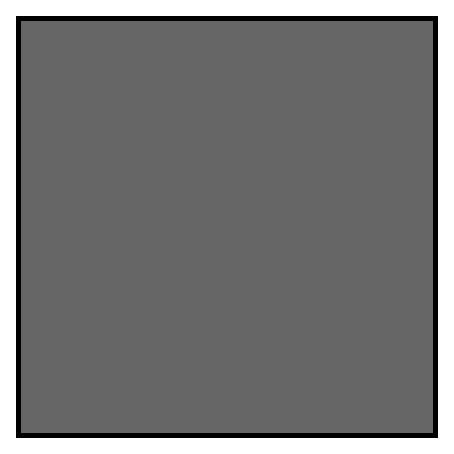
\includegraphics{example.eps}
%% figure caption is below the figure
%\caption{Please write your figure caption here}
%\label{fig:1}       % Give a unique label
%\end{figure}
%%
%% For two-column wide figures use
%\begin{figure*}
%% Use the relevant command to insert your figure file.
%% For example, with the graphicx package use
%  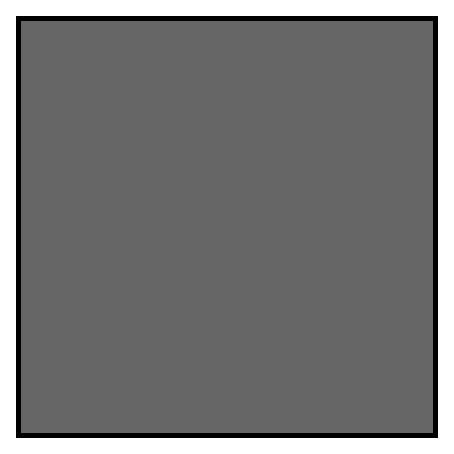
\includegraphics[width=0.75\textwidth]{example.eps}
%% figure caption is below the figure
%\caption{Please write your figure caption here}
%\label{fig:2}       % Give a unique label
%\end{figure*}
%%
%% For tables use
%\begin{table}
%% table caption is above the table
%\caption{Please write your table caption here}
%\label{tab:1}       % Give a unique label
%% For LaTeX tables use
%\begin{tabular}{lll}
%\hline\noalign{\smallskip}
%first & second & third  \\
%\noalign{\smallskip}\hline\noalign{\smallskip}
%number & number & number \\
%number & number & number \\
%\noalign{\smallskip}\hline
%\end{tabular}
%\end{table}


%\begin{acknowledgements}
%If you'd like to thank anyone, place your comments here
%and remove the percent signs.
%\end{acknowledgements}

%\bibliographystyle{spbasic}      % basic style, author-year citations
%\bibliographystyle{spmpsci}      % mathematics and physical sciences
%\bibliographystyle{spphys}       % APS-like style for physics
\bibliographystyle{apalike}
\bibliography{Bibliography}   % name your BibTeX data base

% Non-BibTeX users please use
%\begin{thebibliography}{}
%
% and use \bibitem to create references. Consult the Instructions
% for authors for reference list style.
%
%\bibitem{RefJ}
% Format for Journal Reference
Author, Article title, Journal, Volume, page numbers (year)
% Format for books
%\bibitem{RefB}
Author, Book title, page numbers. Publisher, place (year)
% etc
%\end{thebibliography}

\end{document}
% end of file template.tex

